% !TeX program = lualatex
\documentclass{article}
\usepackage{graphicx} % Required for inserting images
\usepackage{bussproofs} % Added for proof trees
\usepackage{amsthm}
\usepackage{agda}
\usepackage{catchfilebetweentags}
\usepackage{iftex}
\ifLuaTeX\else
  \PackageError{tempM}{This document must be compiled with LuaLaTeX}{Use lualatex (with biber) instead of pdflatex/xelatex.}
\fi
% Use fonts with a decent coverage of non-ASCII characters.
\usepackage{fontspec}
\usepackage{amsmath}
\usepackage{amsfonts}
\usepackage{amssymb}
\usepackage[style=alphabetic,backend=biber]{biblatex}
\addbibresource{references.bib}
\newfontfamily{\AgdaSerifFont}{Latin Modern Roman}
\newfontfamily{\AgdaSansSerifFont}{Latin Modern Sans}
\newfontfamily{\AgdaTypewriterFont}{Latin Modern Mono}
\newfontface{\gearsymbol}{Noto Sans Symbols}
\renewcommand{\AgdaFontStyle}[1]{{\AgdaSansSerifFont{}#1}}
\renewcommand{\AgdaKeywordFontStyle}[1]{{\AgdaSansSerifFont{}#1}}
\renewcommand{\AgdaStringFontStyle}[1]{{\AgdaTypewriterFont{}#1}}
\renewcommand{\AgdaCommentFontStyle}[1]{{\AgdaTypewriterFont{}#1}}
\renewcommand{\AgdaBoundFontStyle}[1]{\textit{\AgdaSerifFont{}#1}}


% Workarounds for the fact that the Latin Modern Sans font does not
% support certain characters. An alternative would be to use another
% font.
\usepackage{newunicodechar}

% Greek letters
\newunicodechar{λ}{\ensuremath{\lambda}}
\newunicodechar{ρ}{\ensuremath{\rho}}
\newunicodechar{ω}{\ensuremath{\omega}}
\newunicodechar{ℓ}{\ensuremath{\ell}}

% Quantifiers and logical symbols
\newunicodechar{∀}{\ensuremath{\forall}}
\newunicodechar{∃}{\ensuremath{\exists}}
\newunicodechar{⊥}{\ensuremath{\bot}}
\newunicodechar{⊤}{\ensuremath{\top}}

% Mathematical symbols
\newunicodechar{ℕ}{\ensuremath{\mathbb{N}}}
\newunicodechar{∅}{\ensuremath{\varnothing}}
\newunicodechar{∘}{\ensuremath{\circ}}
\newunicodechar{∷}{\ensuremath{::}}
\newunicodechar{∙}{\ensuremath{\cdot}}
\newunicodechar{⋁}{\ensuremath{\bigcup}}

% Subscripts and superscripts
\newunicodechar{₁}{\ensuremath{_1}}
\newunicodechar{₂}{\ensuremath{_2}}

% Relations and operators
\newunicodechar{≤}{\ensuremath{\leq}}
\newunicodechar{≥}{\ensuremath{\geq}}
\newunicodechar{≡}{\ensuremath{\equiv}}
\newunicodechar{≟}{\ensuremath{\stackrel{?}{=}}}
\newunicodechar{′}{\ensuremath{'}}

% Lattice operations
\newunicodechar{⊔}{\ensuremath{\sqcup}}
\newunicodechar{⊓}{\ensuremath{\sqcap}}
\newunicodechar{⋎}{\ensuremath{\curlyvee}}

% Logical connectives
\newunicodechar{∧}{\ensuremath{\land}}
\newunicodechar{∨}{\ensuremath{\lor}}
\newunicodechar{⇒}{\ensuremath{\Rightarrow}}
\newunicodechar{⊎}{\ensuremath{\uplus}}

% Modal operators
\newunicodechar{□}{\ensuremath{\Box}}
\newunicodechar{♢}{\ensuremath{\Diamond}}

% Greek letters (Agda code snippets)
\newunicodechar{α}{\ensuremath{\alpha}}
\newunicodechar{β}{\ensuremath{\beta}}

% Semantic relations
\newunicodechar{⊧}{\ensuremath{\models}}
\newunicodechar{⊪}{\ensuremath{\Vdash}}
\newunicodechar{⊩}{\ensuremath{\Vdash}}
\newunicodechar{⊢}{\ensuremath{\vdash}}

\newunicodechar{≢}{\ensuremath{\not\equiv}}
\newunicodechar{Γ}{\ensuremath{\mathnormal{\Gamma}}}
\newunicodechar{Δ}{\ensuremath{\mathnormal{\Delta}}}
\newunicodechar{δ}{\ensuremath{\mathnormal{\delta}}}
\newunicodechar{∉}{\ensuremath{\notin}}
\newunicodechar{∪}{\ensuremath{\cup}}
\newunicodechar{⚙}{{\gearsymbol ⚙}}

\usepackage{xcolor}
\usepackage{soul}
\usepackage[colorinlistoftodos]{todonotes}
\usepackage[colorlinks=true,linkcolor=blue,urlcolor=teal]{hyperref}

% Agda formalisation links
\newcommand{\agdaBaseUrl}{https://eapiova.github.io/s4dot2-cut-elimination}  % Agda HTML hosted via GitHub Pages
\newcommand{\agdalink}[1]{\href{\agdaBaseUrl/#1}{\raisebox{-0.1em}{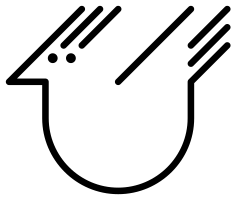
\includegraphics[height=0.9em]{agda-bird}}}}




\newcommand{\seq}[2]{{#1} \vdash{} {#2}}
\newcommand{\pf}[2]{{#1}^{#2}} % Position-formula (superscript)
\newcommand{\mset}[1]{\{#1\}} % Multiset notation for contexts if needed
\newcommand{\cana}[1]{#1\!-\!\pf{A}{s}} 
\newcommand{\logic}{\mathsf{S4.2}}
\newcommand{\calculus}{\mathsf{E}_{\logic}}
\newcommand{\axname}[1]{\mathsf{#1}}
\newcommand{\commento}[1]{}
\newcommand{\eseq}{\mathsf{E}_{{\textsf{S4.2}}}}
\newcommand{\agda}{\textsf{Agda}}
\newcommand{\mform}{\mathcal{MF}}
\newcommand{\pform}{\mathcal{PF}}

\newcommand{\cubical}{\textsf{Cubical Agda}}
\newcommand{\hilbertlogic}[1]{\mathsf{H}_{#1}}

\newtheorem{lemma}{Lemma}[section]
\newtheorem{theorem}{Theorem}[section]
\newtheorem{corollary}{Corollary}
\newtheorem{example}{Example}
\newtheorem{remark}[theorem]{Remark}
\theoremstyle{definition}
\newtheorem{definition}{Definition}[section]
%\title{An Agda Implementation of the Modal Logic S4.2: Theory and Applications}
\title{Metamathematics of the Modal Logic S4.2 in the \agda{} Proof Assistant}
\author{
  Riccardo Borsetto\thanks{Department of Computer Science, University of Verona, Italy.
    Email: \texttt{riccardo.borsetto@univr.it}.} \and
  Margherita Zorzi\thanks{Department of Computer Science, University of Verona, Italy.
    Email: \texttt{margherita.zorzi@univr.it}.}
}
\date{2025}

\begin{document}

\maketitle

\begin{abstract}
    We propose an implementation in the \agda{}~proof assistant of a new deductive system for the modal logic $\logic$. $\logic$ extends $\axname{S4}$ with the axiom $\Diamond\Box\phi \rightarrow \Box\Diamond\phi$ and arises as the underlying logic in different fields, from mathematics to philosophy.
    Despite its widespread applications, $\logic$ has been under-investigated (with respect to other modal systems) for several years. In this paper we focus on the implementation of the metatheory of $\mathsf{E}_{\logic}$, a sequent calculus for $\logic$ built on previous investigations, where formulae are equipped with a \emph{position}, i.e. a set of uninterpreted tokens used to manage modal information. The calculus is designed to enjoy strong proof-theoretic properties, such as a direct syntactic proof of cut elimination, which in turn yields consistency of the system and the subformula property. We implement in \cubical{} both the system and the proof of the Cut-Elimination Theorem. Moreover, we propose the implementation of a constructive version of a semantics for $\logic$ based on semilattices, and we prove a constructive soundness theorem for $\mathsf{E}_{\logic}$ establishing, relying on Segerberg's finite model property, the (almost) constructive equivalence between the Hilbert-style axiomatisation and the sequent calculus.
    This work represents, in perspective, the initial step toward the (still unknown) intuitionistic version of $\logic$ as well as its purely constructive metamathematics.
\end{abstract}

\vspace{1em}
\noindent\textbf{Keywords:} modal logic; S4.2; sequent calculus; cut elimination;
position-based semantics; Cubical Agda; constructive metamathematics;
proof assistants.

\vspace{0.5em}
\noindent\textbf{2020 Mathematics Subject Classification:}
03B45 (modal logic),
03F05 (cut elimination and normal-form theorems),
03B35 (mechanization of proofs and logical operations),
03B70 (logic in computer science).


\section{Introduction}\label{sec:introduction}

\commento{
\fbox{da qui alla prossima nota possiamo anche togliere, intanto lascio}
Cut elimination is a central result in proof theory: it guarantees that every provable formula --- a theorem --- admits a proof that uses only subformulae of the theorem itself. In sequent calculi this means that the proof only uses subformulae of the end-sequent in the derivation tree. Beyond its intrinsic proof-theoretic interest, cut elimination entails as corollaries the (syntactic proof of) consistency of the system and the subformula property, which are essential for proof search and decidability investigations. Last but not least, Cut Elimination carries a strong computational meaning, elevating proofs as computational objects.

While cut elimination for propositional and first-order classical logic is well established, the situation for modal logics-requires dedicated techniques, due to the interplay between modal operators and the structural management of contexts.
On the one side, the transition to first-order to modal logic is quite natural if one exploit the analogy between modal operators and quantifiers; on the other hand, manage modal information is challenging (see the archetypical case of $\axname{S4}$) and many solutions have been introduced ad hoc for specific systems, by loosing modularity and sometimes also the elegant analogy modalities-quantifiers cited above.
In the last decades, modal proof-theory canalized a renewed interested  and several extensible deductive frameworks with strong properties have been defined and studied (see Section~\ref{sec:related}).
The flourishing of  deductive systems and the interesting relationships among different approaches have raised new questions not only regarding the most studied systems—the so-called normal extensions of logic $\axname{K}$---but also regarding substructural logics and systems intermediate between $\axname{S4}$ and $\axname{S5}$. Our work investigate this latter family of logics and in particular addresses the system $\logic$ by following a ``geometric'' approach to modal proof theory.

\fbox{fin qui, mettendo due righe introduttive direttamente su $\logic$}
}

%\subsection{On the Logic $\logic$}
$\logic$ is a normal modal system that extends $\axname{S4}$ with the Geach axiom $\Diamond\Box\phi \rightarrow \Box\Diamond\phi$ that, in terms of the Sahlqvist correspondence, forces the Church-Rosser property on the relation in the subtended Kripke models. $\logic$ enjoys a number of interesting and heterogeneous instances.

One of the important ones is in the formalisation of temporal reasoning. As investigated by Goldblatt~\cite{Goldblatt1980:Diodorean}, if one interprets modal necessity $\Box$ in the Diodorean sense as ``it is true now and will always be the case that,'' and possibility $\Diamond$ as ``it is true now or will be true at some future time,'' then within the framework of $n$-dimensional Minkowski spacetime (for $n \geq 2$), the mathematical setting of special relativity, the set of valid modal sentences is precisely the logic S4.2. %The temporal ordering in this context, where an event $y$ is in the future of $x$ if a signal can travel from $x$ to $y$ at or below the speed of light, is reflexive and transitive (validating axioms T and 4). Crucially, this ordering is also directed: any two events share a common future event. This directedness property of the causal future is what validates the Geach axiom G, thereby establishing S4.2 as the logic of this relativistic temporal interpretation.

Another fundamental area where S4.2 plays a pivotal role is in the modal logic of set-theoretic forcing, a powerful technique developed by Paul Cohen to prove the independence of the Continuum Hypothesis and other statements from ZFC set theory. Hamkins and L\"owe~\cite{Hamkins2008:ModalForcing} explored the principles governing truth across forcing extensions when modal operators are interpreted as follows: $\Box\phi$ means ``$\phi$ holds in all forcing extensions,'' and $\Diamond\phi$ means ``$\phi$ holds in some forcing extension.'' They demonstrated that, assuming ZFC is consistent, the ZFC-provable principles of forcing under this interpretation are exactly the theorems of S4.2. %The axioms K, T, and 4 are relatively straightforward to verify. The Geach axiom G is validated by the inherent directedness of the forcing relation: given any two forcing conditions, there exists a common extension (e.g., via product forcing), ensuring that if something is possibly necessary, it is necessarily possible. Their proof ingeniously uses ``button'' and ``switch'' sentences within models of set theory (like L) to simulate finite S4.2 Kripke models, thereby showing that any non-S4.2 theorem can be falsified in some model of ZFC.

The reach of S4.2 extends further into abstract algebra. Berger, Christensen Block, and L\"owe investigated ``the modal logic of abelian groups''~\cite{Berger2023:ModalAbelian}, where worlds are abelian groups and the accessibility relation $A \leq B$ signifies that group $A$ is isomorphic to a subgroup of group $B$. Under this interpretation, $\Box\phi$ means $\phi$ holds in all supergroups (up to isomorphism), and $\Diamond\phi$ means $\phi$ holds in some supergroup. Their main result establishes that the modal logic of the class of all abelian groups under this subgroup relation is precisely S4.2. %The reflexivity and transitivity of the subgroup relation validate axioms T and 4. The directedness property, crucial for axiom G, is satisfied because any two abelian groups $A$ and $B$ can be embedded into their direct product $A \times B$, which serves as a common supergroup. The proof again employs a sophisticated adaptation of the button and switch technique, using properties of prime order elements and divisibility to demonstrate the independence required to show that the logic is no stronger than S4.2.

Despite this wide range of applications, with respect to other systems, $\logic$ is less investigated, both from a theoretical and an implementation-oriented perspective (see Section~\ref{sec:related} for a survey of related deductive systems and implementations). In particular, since the intuitionistic axiomatisation of $\logic$ is not known, its computational aspects remain unexplored. To deepen its metatheoretical properties seems to have a twofold interest: to advance in the knowledge of $\logic$ proof theory and, through the implementation, try to understand the classical content of the proofs, possibly moving towards a purely constructive metatheory.

\subsection{Our Contribution, from theory to implementation}
In this present paper we do the first step in the direction sketched above by focusing on the implementation and building on our previous investigation in natural deduction. We propose and implement a new deductive system for $\logic$ called $\eseq$ as a version of \emph{2-sequent}s. 2-sequents have been originally introduced and developed in~\cite{Masini1992:TwoSequentModalities, Masini1993:TwoSequentIntuitionism,MM:ONFineStr:95,MM:ComInt:95} where the authors showed how to characterize the negative $\bot$-free fragments of the modal logics $\axname{K}$, $\axname{T}$, $\axname{K4}$ and $\axname{S4}$, and for the corresponding Multiplicative Exponential Linear Logic (MELL) subsystems. The idea has been successively refined in~\cite{GMM:an-exp-ext-seq,GueMarMasPNGC2001} extending the approach to deal with the full MELL (and other linear systems) both in sequent calculi, and proof nets. More recently, they are further expanded in~\cite{Martini2023:CutElimination}, where an extensible system covering the classical modal logics in the $\axname{K}$, $\axname{D}$, $\axname{T}$, $\axname{K4}$, $\axname{D4}$ and $\axname{S4}$ spectrum is studied. We build in particular on this latter version of 2-sequents and on a natural deduction system counterpart introduced for $\logic$ in~\cite{Martini2024:S42NaturalDeduction}.
The leading idea of this modal  proof-theory style is to decorate formulae with modal information, called \emph{position}, adding a spatial extension to the proof system.
As shown in~\cite{Martini2023:CutElimination}, by interpreting positions as \emph{lists} of uninterpreted tokens (then forcing a notion of positionality and multiplicity), one can characterise different systems by ``tuning'' some constraints on modal rules in a rule system shared by all the logics in the framework. According to~\cite{Martini2024:S42NaturalDeduction}, lists for positions are too structured to capture the intermediate system $\logic$, and the correct choice is to move to a notion of \emph{set-positions}, where positions are simply sets of tokens.

The sequent calculus $\eseq$ for $\logic$ we present, study and implement, enjoys some strong structural properties. Our main result is the Cut-Elimination Theorem, fully formalised in the \agda{} proof assistant, from which the consistency of the system and the Subformula Property follow as corollaries, by purely syntactic arguments. We also present the implementation of a direct proof of the Subformula Property.% Moreover, $\eseq$ is complete w.r.t. the Hilbert-style axiomatisation of $\logic$ and it is also s

%Before proceeding, it is appropriate to make a remark. The transition from natural deduction to the sequent calculus (and conversely) is by no means automatic. There are well-known and significant examples in which a logic (or a family of logics) admits a satisfactory formulation in one framework, while the other remains problematic. This is the case, for instance, with Linear Logic, for which no fully satisfactory system of natural deduction has been developed. In the case of $\logic$, the transition is natural; however, it is by no means technically trivial.

%---and in particular for intermediate systems between $\axname{S4}$ and $\axname{S5}$--
The use of (set-)positions to track modal information always introduces specific challenges, for example the cut elimination proof must account for token freshness, position substitution, and the interaction between eigenpositions and the Geach axiom. As a consequence, the proofs of the theorems are not a simple rework of our previous work and, in particular, their embedding in $\cubical$ requires a careful approach (we discuss below how we choose $\cubical$ among the other proof-assistants).

We list here the main properties of $\eseq$ that guide both the theoretical design and the embedding in $\cubical$:

\begin{itemize}
    \item

Following the approach of 2-sequents, we do not need an explicit formalisation of the accessibility relation as in labelled systems~\cite{Negri:2011, Basin1998:NonClassical}: positions act as a kind of spatial coordinates that provide ``geometrical'' information to formulae.

\item We fully exploit the formal proof-theoretical analogy between first-order quantifiers and modal connectives: we treat the $\Box$ and $\Diamond$ operators as the universal and the existential quantifiers, also retracing the usual constraints to avoid the capture of variables, here redefined w.r.t.\ tokens.
\item We have exactly one right and one left rule for each modal connective; only modal operators can change the position of formulae; logical connectives can be applied only to formulae living at the same position.

\end{itemize}


Let us now turn to the choices on the implementation side. As already emphasised, the proof theory of modal logic is far from trivial, and the correct management of modal information within proofs makes the proofs themselves highly complex.
The complexity of the proofs, in particular the proofs of the Cut-Elimination and related results, motivates the use of a proof assistant to verify the metatheory.


We adopt a deep embedding approach, whereby the syntax and inference rules of $\eseq$ are explicitly represented within the proof assistant. This methodology enables us to formally establish theorems about $\eseq$ and to reason precisely about the logical content of proofs concerning its metatheory.





\subsection{Why Cubical \agda?}
We carry out our formalisation in \emph{Cubical \agda}~\cite{VMA2021:CubicalAgda,AgdaTeam2025:Documentation}, an extension of \agda{} that replaces axiom-based propositional equality with a computational one grounded in cubical type theory.
In the syntactic core presented in this paper, the \textsf{agda/cubical} library is used mainly as a convenient infrastructure: \texttt{Cubical.Data.DescendingList.Strict} provides the sorted descending lists (SDL) we use to represent positions; \texttt{Cubical.Algebra.Semilattice} supplies the algebraic framework for our semantic models; and the basic data types (\texttt{Cubical.Data.List}, \texttt{Sum}, \texttt{Sigma}, \texttt{Nat}, \texttt{Bool}) are imported throughout.
The one Cubical-specific feature actively exploited in the current development is the higher inductive type \texttt{HITs.ListedFiniteSet} (\texttt{LFSet}), whose path constructors give us decidable, quotiented set equality essentially for free; we use it in \texttt{SortedPosition} and \texttt{System} to discharge SDL set-equality lemmas that would otherwise require a setoid construction.

Compared to tactic-based proof assistants such as Coq, Lean, or Isabelle, \agda{}'s functional, proof-term--oriented approach and Unicode syntax keep formalised definitions close to their mathematical presentations, particularly advantageous for a system in which the manipulation of positions plays a central role.
Moreover, \agda{}'s constructive foundation naturally complements the proof-theoretic orientation of this work and supports future extensions toward an intuitionistic version of $\logic$ (Section~\ref{sec:conclusions_future}).

The deeper motivation for committing to \emph{Cubical} \agda{}, rather than to standard \agda, lies in the broader research programme.
The planned semantic explorations, constructive variants of the semilattice semantics, the intuitionistic version of $\logic$, abelian-group semantics following~\cite{Berger2023:ModalAbelian}, and the $\mathsf{NAMOR}$ framework spanning the spectrum of normal modal logics, will require features that are unavailable constructively in standard \agda: definitional function extensionality, for comparing semantic interpretations as functions over (possibly infinite) carriers without postulates; computational univalence, so that isomorphic frames or models can be treated as equal without an axiomatic transport; and higher inductive types for quotienting frames or models by p-morphisms or by truth-equivalence.
By building the syntactic core on cubical foundations now, these semantic extensions will be drop-in additions rather than requiring a foundation switch (see Section~\ref{sec:conclusions_future}).

\textbf{Outline of the paper.}
Section~\ref{sec:calculus} introduces the sequent calculus $\calculus$, including positions, position-formulae, the inference rules, and weak completeness w.r.t.\ the Hilbert-style axiomatisation.
Section~\ref{sec:cutelim} presents the cut elimination theorem, with its proof and \agda{} implementation.
Section~\ref{sec:finite-semantics} describes the finite semilattice semantics, the constructive soundness theorem, and the Hilbert--sequent equivalence.
Section~\ref{sec:related} surveys related work.
Section~\ref{sec:conclusions_future} discusses conclusions and future directions.

\medskip

\textbf{Guide to the reading.} The reader can access the complete \agda{} code through the symbol ``\agdalink{}''. When particularly meaningful, we also include and comment on excerpts of the code along the paper.



%%%%%%%%%%%%%%SISTEMA, REGOLE, WEAK COMPLETENESS%%%%%%%%%%%%%%%%%
\section{The sequent calculus \texorpdfstring{$\calculus$}{E\_S4.2}}\label{sec:calculus}

In this section we present the syntax, the deductive system and the Weak Completeness Theorem w.r.t.\ a standard Hilbert-style axiomatisation of $\logic$.



We start from the ground notion of token, position and position-formula.
As mentioned in the introduction, we will label formulae with sets of uninterpreted tokens.


\begin{definition}[Tokens \agdalink{S4dot2.SortedPosition.html\#Token}]
We assume to have a countable set $\mathcal{T}=\{x_0,x_1,\ldots\}$ of tokens ranged by meta-variables $x,y,z$, possibly indexed.
We use juxtaposition (with an infix comma) for set-theoretic union:
a finite set of tokens $\{x_1,\ldots,x_n\}$ is represented by $x_1,\ldots,x_n$;
with $s,t$ we denote $s\cup t$ and with $s,x$ we denote $s\cup\{x\}$.
 $\varnothing$ denotes the empty set, and therefore
$s,\varnothing=\varnothing, s= s$.
\end{definition}




\begin{definition}[Positions \agdalink{S4dot2.SortedPosition.html\#Position}]
We call \emph{set-position} (or, briefly, \emph{position}) any finite and possibly empty set of tokens. Let $\mathcal{P}$ be the set of positions, ranged by metavariables $s,t,u$ possibly indexed.
%We begin by defining the syntax of $\mathsf{E}_{{\textsf{S4.2}}}$.   %This includes the underlying logical language, the notions of tokens and positions, and finally, position-formulae and position-sequents themselves.
\end{definition}


The language $\mathcal{L}$ consists of a countably infinite set of propositional symbols $p_0, p_1, \dots$, propositional connectives $\wedge, \vee, \rightarrow, \neg$, modal operators $\Box, \Diamond$ and auxiliary symbols $(, )$.
All propositional connectives and both modal operators are taken as primitive, rather than being inter-defined, in order to give each its own left and right introduction rules in the sequent calculus, mirroring the standard presentation in the literature. 
This choice is also forward-looking: in the planned intuitionistic version of $\logic$ (Section~\ref{sec:conclusions_future}), the classical inter-definability of connectives (e.g., $A \vee B = \neg(\neg A \wedge \neg B)$, $\Diamond A = \neg \Box \neg A$) breaks down, so having each connective primitive from the outset means the syntactic core can be reused without restructuring the formula type. 



Our main syntactic objects are the \emph{position-formulae}, i.e.\ modal formulae labelled by positions.


\begin{definition}[Formulae \agdalink{S4dot2.Syntax.html\#Formula}]
    The set $\mform$  of \textit{modal formulae}
    of ${\mathcal L}$ is the least set that contains the propositional
    symbols and is closed under application of the propositional
    connectives and the modal operators.
A formula is atomic if it is a propositional symbol. Negation $\neg$ is taken as a primitive connective.
\end{definition}

\begin{definition}[Position Formulae \agdalink{S4dot2.Syntax.html\#PFormula}]
A \textit{position-formula} (briefly \textit{p-formula}) is an expression of the form $\pf{A}{s}$, where
        $A$ is a modal formula and $s \in \mathcal{P}$. $\pform$ is the set of position-formulae.
\end{definition}

The use of \emph{sets} of tokens for positions is a key feature of $\calculus$, distinguishing it from earlier extended sequent calculi that typically employed \emph{sequences} of tokens~\cite{Martini2023:CutElimination}. This choice, introduced in~\cite{Martini2024:S42NaturalDeduction} for natural deduction, aligns naturally with the semilattice semantics of $\logic$: positions represent finite collections of modal constraints without an artificial ordering and multiplicity, and the union operation ($s,t$ or $s,x$) reflects the join in a semilattice with minimum. This is crucial for capturing the confluence (weak directedness) property that characterises $\logic$ frames.

%We need sometimes to replace tokens inside positions.  Given a token $x$ and positions $s$ and $t$, the \emph{substitution} $s[x/t]$ is defined as $
%s[x/t]=(s\setminus \{x\}) \cup t \quad \mbox{if\ } x \in s$ and 
%$s$ otherwise.

\bigskip 

A token is defined in the proof assistant as a natural number (an element in the set $\mathbb{N}$). This provides a countably infinite supply of names without requiring a fixed bound parameter. Decidable equality on $\mathbb{N}$ (\textsf{discreteℕ} from the \textsf{agda/cubical} library~\cite{VMA2021:CubicalAgda}) enables implementing ``freshness'' constraints in the modal rules, which require introducing a token not previously used in a given context: a fresh token is obtained by taking one more than the maximum token occurring in the current context.

A position is implemented as a \emph{sorted descending list} (SDL) of tokens, a data structure from the \textsf{agda/cubical} library that provides a canonical representation of finite sets. The SDL representation guarantees no duplicates and a fixed ordering, yielding decidable equality and membership. Set operations, union (\textsf{merge}), membership ($\in$), subset ($\subseteq$), are all decidable.

\bigskip 

\commento{
\begin{definition}
    Given a token $x$ and positions $s$ and $t$, the \emph{substitution} $s[x/t]$ is defined as
    \[
s[x/t]=
\begin{cases}
(s\setminus \{x\}) \cup t \quad \mbox{if\ } x \in s
\\
s \quad\mbox{otherwise.}
\end{cases}
\]
\end{definition}
}



%\ExecuteMetaData[Chapter2.tex]{pf}

Position sequents naturally expand the usual notion of sequents as tuples of finite sequences of p-formulae:

\begin{definition}[\agdalink{S4dot2.Syntax.html\#Sequent}]\label{def:extseq}
A \emph{position sequent} (e-sequent) is an expression $\seq{\Gamma}{\Delta}$, where $\Gamma$ and $\Delta$ are finite sequences of p-formulae.
\end{definition}

%\ExecuteMetaData[Chapter2.tex]{eseq}

The notions of \emph{subformula} and \emph{degree} are defined in a (quite) usual way. Observe that, as the set of first-order (Gentzen) subformulae of $\forall x A(x)$ contains all the term-instances of $A(x)$, here the set of (position, modal) subformulae of $\pf{\Box A}{\alpha}$ contains all the extensions of the position $\alpha$ in $\pf{A}{\alpha}$.

\begin{definition}[Subformulae \agdalink{S4dot2.CutElimination.SubformulaProperty.html\#_isSubformulaOf_}]\label{def:subform}
    The set $Sub(\pf{A}{s})$ of subformulae of a p-formula $\pf{A}{s}$ is defined recursively:
\begin{itemize}
    \item $Sub(\pf{p}{s}) = \{\pf{p}{s}\}$ if $p$ is a propositional symbol or $\bot$.
    \item $Sub(\pf{\neg A}{s}) = \{\pf{\neg A}{s}\} \cup Sub(\pf{A}{s})$.
    \item $Sub(\pf{A \circ B}{s}) = \{\pf{A \circ B}{s}\} \cup Sub(\pf{A}{s}) \cup Sub(\pf{B}{s})$ for $\circ \in \{\wedge, \vee, \rightarrow\}$.
    \item $Sub(\pf{\Box A}{s}) = \{\pf{\Box A}{s}\} \cup \bigcup_{t \in \mathcal{P}} Sub(\pf{A}{s,t})$.
    \item $Sub(\pf{\Diamond A}{s}) = \{\pf{\Diamond A}{s}\} \cup \bigcup_{t \in \mathcal{P}} Sub(\pf{A}{s,t})$.
\end{itemize}
\end{definition}
Note: This definition implies that $\pf{A}{s,t}$ is a subformula of $\pf{\Box A}{s}$ for any position $t$.



 In Section~\ref{sec:cutelim} we also introduce a standard notion of degree of a formula and rank of a proof, according to the number of the cut-formulae.



%\subsection{Position Substitution and Renaming}
%The notation $\Gamma[x/t]$ (or $\Delta[x/t]$) means applying this substitution to all positions in all p-formulae in $\Gamma$ (or $\Delta$).

\subsection{The Hilbert Style Formulation of \texorpdfstring{$\logic$}{S4.2}}

We briefly recall the axiomatic (``Hilbert-style'') presentation of the logic \textbf{S4.2}, given over the language with all propositional connectives $\neg, \wedge, \vee, \to$ and both modal operators $\Box, \Diamond$ as primitive (in line with the syntactic choice discussed above).
%In Section \label{sec:completeness} we prove the completeness of our natural deduction system with respect to the Hilbert-style axiomatisation of the logic \textbf{S4.2}. We recall axioms and closure rules in the following definition.

\bigskip



\begin{definition}[Hilbert-Style Axiomatisation $\hilbertlogic{\logic}$ \agdalink{S4dot2.Syntax.html\#Axiom}]\label{def:hilbert}

$\hilbertlogic{\logic}$ is the smallest set $X$ of formulae that      contains all instances of the following schemas:

    \begin{description}
        \item[P1]
        $A\to(B \to A)$
        \item[P2] $(A\to (B\to C))\to ((A\to B)\to (A\to C))$
        \item[P3] $((\neg B\to \neg A)\to ((\neg  B\to A)\to B)) $
        \item[K] $\Box(A\to B)\to(\Box A \to \Box B)$
        \item[D] $\Box A \to \Diamond A$
        \item[T] $\Box A \to A$
        \item[4] $\Box A \to \Box\Box A$
        \item[G/.2] $\Diamond\Box A \to \Box\Diamond A$
    \end{description}
 and is closed under the following:
\begin{description}
    \item[MP]  if $A,A\to B \in X$ then $B\in X$;
    \item[NEC] if $A\in X$ then $\Box A\in X$.
\end{description}

\end{definition}
We write $\vdash_{\hilbertlogic{\logic}}  A$  for  $A\in \hilbertlogic{\logic}$. Notice that, in the presence of Axiom \textbf{P3}, the underlying propositional logic is \emph{classical}. The $\axname{D}$ axiom is needed because $\Diamond$ is taken as a primitive connective rather than defined as $\neg\Box\neg$; in the latter case it would be derivable.


\subsection{The Calculus \texorpdfstring{$\calculus$}{E\_S4.2} \texorpdfstring{\agdalink{S4dot2.System.html\#_⊢_}}{}}

In this section we present the Sequent Calculus $\calculus$. 
Observe that, as usual in sequent calculi presentations,  sequences of formulae ($\Gamma$, $\Delta$), or positions ($s$, $t$) \emph{may be empty}, except when explicitly forbidden.
The constraint on necessitation (rule $\vdash\Box$, and its dual $\Diamond\vdash$) is formulated as a constraint on position occurrences in the context, \emph{analogously to the usual constraint on variable occurrences for $\forall$-introduction} ($\exists$-elimination, respectively).


The inference rules of $\mathsf{E}_{{\textsf{S4.2}}}$ are divided into four categories: identity, structural, propositional, and modal rules. The propositional rules are standard, adapted to operate on p-formulae, and act between formulae defined at the same position. Contexts ($\Gamma$, $\Delta$) are represented as lists rather than multisets: lists have native support in \agda, with decidable equality and straightforward inductive definitions, making them the natural choice for the formalisation. The structural rules (Weakening, Contraction, Exchange) are included explicitly, so that the system with list-based contexts is equivalent to a multiset-based presentation. The core of the calculus lies in the modal rules, which manipulate the positions associated with modal formulae.
The rules $\vdash \Box$ and $\Diamond \vdash$ introduce a fresh token $x$ such that $x \notin s$ and $x$ is new to the rest of the sequent. By analogy to first-order sequent calculi, we call respectively \emph{eigenposition} and \emph{eigentoken} the position $s,x$ and the token $x$ in the rules  $\vdash \Box$ and $\Diamond \vdash$.
In first-order sequent calculi, the freshness condition does not affect which end sequents are provable, up to renaming of bound variables, and guarantees that each eigenvariable in a derivation is associated with exactly one right-$\forall$ or left-$\exists$ rule.
% Moreover, that variable occurs in the derivation only above the rule of which
% it is eigenvariable, and it never occurs as a bound variable.
We extend the idea to position sequents (following~\cite{Martini2023:CutElimination}) in the following section, by stating and proving the Token-Position Substitution Lemma~\ref{lem:pos-subst-validity} (which subsumes token renaming as a special case).

%We express this in \agda{}~by means of the following code
%\ExecuteMetaData[Chapter2.tex]{fresh}

 
% where:  given a list $\Gamma$, the operator $\mathsf{pf.s}$ extracts the position from a position formula,  the operator $\mathsf{map}$ applies the extraction to each element of $\Gamma$, $\bigcup$ implements the union of all the positions and $x$ is a new token that satisfies the condition.   


Notice that the freshness condition is analogous to the eigenvariable condition in first-order logic sequent calculi, and ensures that the introduced token represents an arbitrary, new point in the modal context relative to position $s$. The management of these tokens and set positions is crucial for correctly capturing the properties of $\logic$ and proving proof-theoretical results.


We show the rules of $\eseq$. %and the corresponding $Agda$ implementation. See Appendix\ref{appendix:rules} for the complete system.

\subsection*{Identity Rules}
\[
\AxiomC{}
\RightLabel{$Ax$}
\UnaryInfC{$\seq{\pf{A}{s}}{\pf{A}{s}}$}
\DisplayProof
\qquad
\AxiomC{$\seq{\Gamma_1}{\pf{A}{s}, \Delta_1}$}
\AxiomC{$\seq{\Gamma_2, \pf{A}{s}}{\Delta_2}$}
\RightLabel{$Cut$}
\BinaryInfC{$\seq{\Gamma_1, \Gamma_2}{\Delta_1, \Delta_2}$}
\DisplayProof
\]

\subsection*{Structural Rules}
\[
\AxiomC{$\seq{\Gamma}{\Delta}$}
\RightLabel{$W\vdash$}
\UnaryInfC{$\seq{\Gamma, \pf{A}{s}}{\Delta}$}
\DisplayProof
\qquad
\AxiomC{$\seq{\Gamma}{\Delta}$}
\RightLabel{$\vdash W$}
\UnaryInfC{$\seq{\Gamma}{\pf{A}{s}, \Delta}$}
\DisplayProof
\]
\[
\AxiomC{$\seq{\Gamma, \pf{A}{s}, \pf{A}{s}}{\Delta}$}
\RightLabel{$C\vdash$}
\UnaryInfC{$\seq{\Gamma, \pf{A}{s}}{\Delta}$}
\DisplayProof
\qquad
\AxiomC{$\seq{\Gamma}{\pf{A}{s}, \pf{A}{s}, \Delta}$}
\RightLabel{$\vdash C$}
\UnaryInfC{$\seq{\Gamma}{\pf{A}{s}, \Delta}$}
\DisplayProof
\]
\[
\AxiomC{$\seq{\Gamma_1, \pf{A}{s}, \pf{B}{t}, \Gamma_2}{\Delta}$}
\RightLabel{$E\vdash$}
\UnaryInfC{$\seq{\Gamma_1, \pf{B}{t}, \pf{A}{s}, \Gamma_2}{\Delta}$}
\DisplayProof
\qquad
\AxiomC{$\seq{\Gamma}{\Delta_1, \pf{A}{s}, \pf{B}{t}, \Delta_2}$}
\RightLabel{$\vdash E$}
\UnaryInfC{$\seq{\Gamma}{\Delta_1, \pf{B}{t}, \pf{A}{s}, \Delta_2}$}
\DisplayProof
\]

\subsection*{Propositional Rules}
\[
\AxiomC{$\seq{\Gamma, \pf{A}{s}}{\Delta}$}
\RightLabel{$\wedge_1 \vdash$}
\UnaryInfC{$\seq{\Gamma, \pf{A \wedge B}{s}}{\Delta}$}
\DisplayProof
\qquad
\AxiomC{$\seq{\Gamma, \pf{B}{s}}{\Delta}$}
\RightLabel{$\wedge_2 \vdash$}
\UnaryInfC{$\seq{\Gamma, \pf{A \wedge B}{s}}{\Delta}$}
\DisplayProof
\]
\[
\AxiomC{$\seq{\Gamma_1}{\pf{A}{s}, \Delta_1}$}
\AxiomC{$\seq{\Gamma_2}{\pf{B}{s}, \Delta_2}$}
\RightLabel{$\vdash \wedge$}
\BinaryInfC{$\seq{\Gamma_1, \Gamma_2}{\pf{A \wedge B}{s}, \Delta_1, \Delta_2}$}
\DisplayProof
\]
\[
\AxiomC{$\seq{\Gamma_1, \pf{A}{s}}{\Delta_1}$}
\AxiomC{$\seq{\Gamma_2, \pf{B}{s}}{\Delta_2}$}
\RightLabel{$\vee \vdash$}
\BinaryInfC{$\seq{\Gamma_1, \Gamma_2, \pf{A \vee B}{s}}{\Delta_1, \Delta_2}$}
\DisplayProof
\qquad
\AxiomC{$\seq{\Gamma}{\pf{A}{s}, \Delta}$}
\RightLabel{$\vdash \vee_1$}
\UnaryInfC{$\seq{\Gamma}{\pf{A \vee B}{s}, \Delta}$}
\DisplayProof
\]
\[
\AxiomC{$\seq{\Gamma}{\pf{B}{s}, \Delta}$}
\RightLabel{$\vdash \vee_2$}
\UnaryInfC{$\seq{\Gamma}{\pf{A \vee B}{s}, \Delta}$}
\DisplayProof
\]
\[
\AxiomC{$\seq{\Gamma_1}{\pf{A}{s}, \Delta_1}$}
\AxiomC{$\seq{\Gamma_2, \pf{B}{s}}{\Delta_2}$}
\RightLabel{$\rightarrow \vdash$}
\BinaryInfC{$\seq{\Gamma_1, \Gamma_2, \pf{A \rightarrow B}{s}}{\Delta_1, \Delta_2}$}
\DisplayProof
\qquad
\AxiomC{$\seq{\Gamma, \pf{A}{s}}{\pf{B}{s}, \Delta}$}
\RightLabel{$\vdash \rightarrow$}
\UnaryInfC{$\seq{\Gamma}{\pf{A \rightarrow B}{s}, \Delta}$}
\DisplayProof
\]
\subsection*{Modal Rules}
\[
\AxiomC{$\seq{\Gamma, \pf{A}{s,t}}{\Delta}$}
\RightLabel{$\Box \vdash$}
\UnaryInfC{$\seq{\Gamma, \pf{\Box A}{s}}{\Delta}$}
\DisplayProof
\qquad
\AxiomC{$\seq{\Gamma}{\pf{A}{s,x}, \Delta}$}
\RightLabel{$\vdash \Box$}
\UnaryInfC{$\seq{\Gamma}{\pf{\Box A}{s}, \Delta}$}
\DisplayProof
%\quad \text{(Constraint: } x \notin s \text{ and } x \text{ fresh for } \Gamma, \Delta) \text{)}
\]
\[
\AxiomC{$\seq{\Gamma, \pf{A}{s,x}}{\Delta}$}
\RightLabel{$\Diamond \vdash$}
\UnaryInfC{$\seq{\Gamma, \pf{\Diamond A}{s}}{\Delta}$}
\DisplayProof
%\quad \text{(Constraint: } x \notin s \text{ and } x \text{ fresh for } \Gamma, \Delta \text{)}
\qquad
\AxiomC{$\seq{\Gamma}{\pf{A}{s,t}, \Delta}$}
\RightLabel{$\vdash \Diamond$}
\UnaryInfC{$\seq{\Gamma}{\pf{\Diamond A}{s}, \Delta}$}
\DisplayProof
\]

with the constraints:  $x \notin s$ and $x$ fresh for $\Gamma, \Delta$ for $\vdash \Box$  and $\Diamond \vdash$.


We show here the \agda{} implementation of the modal fragment.

\ExecuteMetaData[Chapter2.tex]{modalRules}


%\section{On weak completeness and Semantics}\label{sec:completeness}


\subsection{Weak Completeness}
The system $\eseq$ proves, at any position, all the theorems of the Hilbert-style presentation of $\logic$ (see also~\cite{Martini2024:S42NaturalDeduction}). The derivations below are given at the empty position $\varnothing$; derivability at an arbitrary position $s$ then follows by weakening (rule $W\vdash$ or $\vdash W$) applied to the position structure.



%\section{Weak Completeness: \agda{}~derivations of S4.2 Axioms}\label{appendix:axioms}

Given a Hilbert-style axiomatisation $\hilbertlogic{\logic}$ of $\logic$, one achieves weak completeness by showing that all the theorems derivable in $\hilbertlogic{\logic}$ are also theorems of $\calculus$ and that the derivations are closed under necessitation and modus ponens rules.
The following is the key lemma to prove the main theorem:

\begin{lemma}[\agdalink{S4dot2.Equivalence.HilbertCompleteness.html\#derive-P1}]
\begin{description}
\item The following axioms are derivable in $\calculus$
    \begin{itemize}
        \item[P1]   $ \pf{A\to(B \to A)}{\varnothing}$;
        \item[P2]  $  \pf{(A\to (B\to C))\to ((A\to B)\to (A\to C))}{\varnothing}$;
        \item[P3]   $  \pf{((\neg B\to \neg A)\to ((\neg  B\to A)\to B))}{\varnothing} $;
%       \item $A\land B^\varnothing \leftrightarrow \neg (A \to \neg B)$;
%       \item $A\lor B \leftrightarrow \neg (\neg A \land \neg B)$;     
%       \item  $
%           \pf{\Diamond A \leftrightarrow \neg\Box\neg A}{\varnothing}$;
        \item[K] $ \pf{\Box (A\to B)\to (\Box A \to \Box B)}{\varnothing}$;
        \item[T] $   \pf{ \Box A \to A}{\varnothing}$;
        \item[4] $  \pf{ \Box A \to \Box\Box A}{\varnothing}$;
        \item[G/.2]  $ \pf{\Diamond\Box A\to \Box\Diamond A}{\varnothing}$.
    \end{itemize}
\item The following rules are derivable in $\calculus$
\begin{itemize}
    \item if $\;\vdash \pf{A}{\varnothing}$, then also $\vdash \pf{\Box A}{\varnothing}$ (closure under \textbf{NEC});
    \item  if $\;\vdash \pf{A}{\varnothing}$ and $\vdash \pf{A\to B}{\varnothing}$, then also $\;\vdash \pf{B}{\varnothing}$ (closure under \textbf{MP}).
\end{itemize}  
\end{description}
\end{lemma}

\begin{proof}

We show here that axioms $\axname{P1}, \axname{P2}, \axname{P3}, \axname{K}, \axname{T}, \axname{4}, \axname{G/.2}$ of $\logic$ are derivable at the empty position $\varnothing$.

\commento{
\ExecuteMetaData[Chapter2.tex]{axiom1}

\ExecuteMetaData[Chapter2.tex]{axiom2}

\ExecuteMetaData[Chapter2.tex]{axiom3}
}

%\commento{
\subsection*{Axiom K}
\[
\AxiomC{$\seq{\pf{A}{x}}{\pf{A}{x}}$}
\AxiomC{$\seq{\pf{B}{x}}{\pf{B}{x}}$}
\RightLabel{$\rightarrow \vdash$}
\BinaryInfC{$\seq{\pf{A}{x}, \pf{A \rightarrow B}{x}}{\pf{B}{x}}$}
\RightLabel{$\Box \vdash$}
\UnaryInfC{$\seq{\pf{A}{x}, \pf{\Box(A \rightarrow B)}{\varnothing}}{\pf{B}{x}}$}
\RightLabel{$E\vdash$}
\UnaryInfC{$\seq{\pf{\Box(A \rightarrow B)}{\varnothing}, \pf{A}{x}}{\pf{B}{x}}$}
\RightLabel{$\Box \vdash$}
\UnaryInfC{$\seq{\pf{\Box(A \rightarrow B)}{\varnothing}, \pf{\Box A}{\varnothing}}{\pf{B}{x}}$}
\RightLabel{$\vdash \Box$}
\UnaryInfC{$\seq{\pf{\Box(A \rightarrow B)}{\varnothing}, \pf{\Box A}{\varnothing}}{\pf{\Box B}{\varnothing}}$}
\RightLabel{$\vdash \rightarrow$}
\UnaryInfC{$\seq{\pf{\Box(A \rightarrow B)}{\varnothing}}{\pf{(\Box A \rightarrow \Box B)}{\varnothing}}$}
\RightLabel{$\vdash \rightarrow$}
\UnaryInfC{$\seq{}{\pf{(\Box(A \rightarrow B) \rightarrow (\Box A \rightarrow \Box B))}{\varnothing}}$}
\DisplayProof
\]

%}


%\ExecuteMetaData[Chapter2.tex]{axiomK}

Notice the freshness requirement of $x$ for $\vdash \Box$.
%\commento{
\subsection*{Axiom T}
\[
\AxiomC{$\seq{\pf{A}{\varnothing}}{\pf{A}{\varnothing}}$}
\RightLabel{$\Box \vdash$}
\UnaryInfC{$\seq{\pf{\Box A}{\varnothing}}{\pf{A}{\varnothing}}$}
\RightLabel{$\vdash \rightarrow$}
\UnaryInfC{$\seq{}{\pf{(\Box A \rightarrow A)}{\varnothing}}$}
\DisplayProof
\]
%}
%\ExecuteMetaData[Chapter2.tex]{axiomT}

%\commento{
\subsection*{Axiom 4}
\[
\AxiomC{$\seq{\pf{A}{x,y}}{\pf{A}{x,y}}$}
\RightLabel{$\Box \vdash$}
\UnaryInfC{$\seq{\pf{\Box A}{\varnothing}}{\pf{A}{x,y}}$}
\RightLabel{$\vdash \Box$}
\UnaryInfC{$\seq{\pf{\Box A}{\varnothing}}{\pf{\Box A}{x}}$}
\RightLabel{$\vdash \Box$}
\UnaryInfC{$\seq{\pf{\Box A}{\varnothing}}{\pf{\Box \Box A}{\varnothing}}$}
\RightLabel{$\vdash \rightarrow$}
\UnaryInfC{$\seq{}{\pf{(\Box A \rightarrow \Box \Box A)}{\varnothing}}$}
\DisplayProof
\]

%}

%\ExecuteMetaData[Chapter2.tex]{axiom4}
Notice the freshness requirement on $y$ for the first $\vdash \Box$, and the freshness of $x$ for the second $\vdash \Box$.



\subsection*{Axiom G/.2}

\[
\AxiomC{$\seq{\pf{A}{x,y}}{\pf{A}{x,y}}$}
\RightLabel{$\Box \vdash$}
\UnaryInfC{$\seq{\pf{\Box A}{x}}{\pf{A}{x,y}}$}
\RightLabel{$\vdash \Diamond$}
\UnaryInfC{$\seq{\pf{\Box A}{x}}{\pf{\Diamond A}{y}}$}
\RightLabel{$\vdash \Box$}
\UnaryInfC{$\seq{\pf{\Box A}{x}}{\pf{\Box \Diamond A}{\varnothing}}$}
\RightLabel{$\Diamond \vdash$}
\UnaryInfC{$\seq{\pf{\Diamond \Box A}{\varnothing}}{\pf{\Box \Diamond A}{\varnothing}}$}
\RightLabel{$\vdash \rightarrow$}
\UnaryInfC{$\seq{}{\pf{(\Diamond \Box A \rightarrow \Box \Diamond A)}{\varnothing}}$}
\DisplayProof
\]
  where $y$ is fresh for $\vdash \Box$, and $x$ is fresh for $\Diamond \vdash$. Notice the role the interpretation of positions as a set plays in the derivation, allowing one to manipulate tokens independently from the position in the sequence. Moving to a more structured notion of position, we cannot derive the Geach axiom~\cite{Martini2023:CutElimination}. 

For the characteristic axiom, we also show here the \agda{}~code:
\ExecuteMetaData[PaperCode.tex]{geachAxiom}

\noindent
The proof term mirrors the pen-and-paper derivation.
A private module \texttt{G}, parametrised by the formula $A$, pre-computes the positions used in the proof: $\alpha = \varnothing$, $\beta = \{0\}$, $\gamma = \{1\}$, $\delta = \{0,1\}$.
The blue identifiers are helper lemmas that discharge the side conditions of the modal rules:
\texttt{fresh-$\alpha$-0} and \texttt{fresh-$\alpha$-1} witness that tokens $0$ and $1$ do not occur in the empty position~$\alpha$;
\texttt{TokenFresh-[]} witnesses freshness with respect to an empty context;
\texttt{fresh-$\Delta$-$\Diamond\vdash$} and \texttt{fresh-$\Gamma$-$\vdash\Box$} collect the freshness evidence required by the $\Diamond\vdash$ and $\vdash\Box$ rules, respectively.
Finally, \texttt{ax-subst'} applies a position-substitution lemma to turn an instance of \textsc{Ax} at position~$\delta$ into one at the position required by the surrounding context.
%\subsection{Modus Ponens}
\bigskip

\noindent

Closure under Necessitation and Modus Ponens is also clearly derivable. We directly show the \agda{}~code:
\ExecuteMetaData[PaperCode.tex]{NEC}
\noindent
The proof of Necessitation applies the $\vdash\Box$ rule to the hypothesis \texttt{pA}.
A private module \texttt{N}, parametrised by a formula $A$ and a proof \texttt{pA} of $\vdash A^{\varnothing}$, computes a fresh eigentoken \texttt{xN} as the successor of the maximum token occurring in \texttt{pA} (via \texttt{maxEigenposToken}).
The key step is \texttt{liftedN}, which uses \texttt{lift-proof} to transport the derivation \texttt{pA} from position $\varnothing$ to the eigenposition $\{$\texttt{xN}$\}$ required by the premise of $\vdash\Box$; the proof \texttt{ncN} certifies that the eigentoken does not interfere with any eigenposition already used in \texttt{pA}.
Modus Ponens is a direct application of the Cut rule:
\ExecuteMetaData[PaperCode.tex]{MP}

\end{proof}

We can state the Weak Completeness Theorem as an easy corollary of the previous lemma:

\begin{theorem}[Weak Completeness for $\eseq$ \agdalink{S4dot2.Equivalence.HilbertCompleteness.html\#completeness}]\label{th:weakcompleteness}

For each position $s$, if $\vdash_{\hilbertlogic{\logic}} A$ then $\vdash_{\eseq} A^s$.

\end{theorem}


%\section{Some proof-theoretical results}
%\subsection{Preliminaries}
\section{Cut-Elimination for \texorpdfstring{$\eseq$}{E-S4.2}}\label{sec:cutelim}
We propose now our main proof-theoretical result, the Cut Elimination Theorem for $\calculus$.

We start with a central auxiliary lemma. In position-based sequent calculi token and position handling plays a crucial technical role.  We extend some results from~\cite{Martini2023:CutElimination} that allow one to soundly replace tokens with positions inside proofs. As a special case, an eigen-token $x$ in a proof $\Pi$ can be consistently renamed to a fresh token $y$ by substituting $x$ with the singleton position $\{y\}$, resulting in a valid proof $\Pi'$.

%\subsection{Substitution Lemmata}\label{ssec:subst-lemmata}

\commento{
\begin{lemma}[Token Renaming \agdalink{S4dot2.CutElimination.ProofSubst.html\#renameEigenpos-♢⊢-premise-gen}]\label{lem:token-renaming}
Let $\Pi$ be a proof of an e-sequent $\seq{\Gamma}{\Delta}$. Let $x$ be a token, and let $y$ be a token such that $y$ does not occur in any position in $\Pi$ (if $x$ occurs in $\Pi$, this implies $y \neq x$).
Let $\Pi[x \mapsto y]$ denote the proof structure obtained by replacing every occurrence of the token $x$ with the token $y$ within every position $s'$ in $\Pi$. That is, for any position $s'$, $s'[x \mapsto y]$ is defined as $(s' \setminus \{x\}) \cup \{y\}$ if $x \in s'$, and $s'[x \mapsto y] = s'$ if $x \notin s'$.
Similarly, $\Gamma[x \mapsto y]$ and $\Delta[x \mapsto y]$ denote the application of this substitution to all positions in $\Gamma$ and $\Delta$, respectively.
Then, $\Pi[x \mapsto y]$ is a valid proof in $\mathsf{E}_{{\textsf{S4.2}}}$ of the e-sequent $\seq{\Gamma[x \mapsto y]}{\Delta[x \mapsto y]}$.
\end{lemma}


\begin{proof}
The proof proceeds by induction on the height $h(\Pi)$ of the proof $\Pi$.

\begin{description}
    \item[Base Case ($h(\Pi)=1$):] If $\Pi$ is an axiom, e.g., $\seq{\pf{A}{s_0}}{\pf{A}{s_0}}$. Then $\Pi[x \mapsto y]$ is the sequent $\seq{\pf{A}{s_0[x \mapsto y]}}{\pf{A}{s_0[x \mapsto y]}}$, which is still a valid axiom.

    \item[Inductive Step:] Assume the lemma holds for all proofs of height less than $h(\Pi)$. Let $R$ be the last inference rule applied in $\Pi$. We show that applying $R$ to the premise(s) transformed by $[x \mapsto y]$ (which are valid proofs by the induction hypothesis, IH) yields the transformed conclusion, and that all side conditions of $R$ remain satisfied.

    \begin{enumerate}
        \item \textbf{Propositional, Structural, and Cut Rules:} These cases are straightforward. The logical structure of the rules is unaffected. Positions $s_i$ in the premises and conclusion are consistently transformed to $s_i[x \mapsto y]$. For example, if $R$ is $(\wedge \vdash_1)$ from $\seq{\Sigma_0, \pf{A}{s_0}}{\Delta_0}$ to $\seq{\Sigma_0, \pf{A \wedge B}{s_0}}{\Delta_0}$, by IH the premise proof of $\seq{\Sigma_0[x \mapsto y], \pf{A}{s_0[x \mapsto y]}}{\Delta_0[x \mapsto y]}$ is valid. Applying $(\wedge \vdash_1)$ yields $\seq{\Sigma_0[x \mapsto y], \pf{A \wedge B}{s_0[x \mapsto y]}}{\Delta_0[x \mapsto y]}$, which is the correctly substituted conclusion.

        \item \textbf{Modal Rules:}
        \begin{itemize}
            \item Rules $\Box \vdash$ and $\vdash \Diamond$:
            These rules do not have eigen-token side conditions related to the introduced position part.
            For $(\Box \vdash)$, if the premise is $\seq{\Sigma_0, \pf{A}{s_0,u}}{\Delta_0}$ and conclusion $\seq{\Sigma_0, \pf{\Box A}{s_0}}{\Delta_0}$, the transformed premise (by IH) is $\seq{\Sigma_0[x \mapsto y], \pf{A}{(s_0,u)[x \mapsto y]}}{\Delta_0[x \mapsto y]}$. Applying $(\Box \vdash)$ yields $\seq{\Sigma_0[x \mapsto y], \pf{\Box A}{s_0[x \mapsto y]}}{\Delta_0[x \mapsto y]}$. This is correct as $(s_0,u)[x \mapsto y] = (s_0[x \mapsto y], u[x \mapsto y])$. The argument for $(\vdash \Diamond)$ is analogous.

            \item Rule $(\vdash \Box)$: Suppose $\Pi$ ends with $\seq{\Sigma}{\pf{\Box A}{s_0}, \Lambda}$ derived from $\Pi_{prem}: \seq{\Sigma}{\pf{A}{s_0,z}, \Lambda}$, where $z$ is the eigen-token, $z \notin s_0$, and $z$ is fresh for $\Sigma, \Lambda$.
            By IH, $\Pi_{prem}[x \mapsto y]$ is a valid proof of $\seq{\Sigma[x \mapsto y]}{\pf{A}{(s_0,z)[x \mapsto y]}, \Lambda[x \mapsto y]}$.
            We consider two cases for the eigen-token $z$:
            \begin{enumerate}
                \item If $z = x$ (the eigen-token itself is being renamed): The new eigen-token is $y$. The transformed premise formula is $\pf{A}{(s_0,x)[x \mapsto y]} = \pf{A}{s_0[x \mapsto y],y}$. The rule application becomes:
                \[
                \AxiomC{$\seq{\Sigma[x \mapsto y]}{\pf{A}{s_0[x \mapsto y],y}, \Lambda[x \mapsto y]}$}
                \RightLabel{$\vdash \Box$}
                \UnaryInfC{$\seq{\Sigma[x \mapsto y]}{\pf{\Box A}{s_0[x \mapsto y]}, \Lambda[x \mapsto y]}$}
                \DisplayProof
                \]
                Side conditions for $y$:
                (a) $y \notin s_0[x \mapsto y]$: The original condition was $x \notin s_0$. If $x \in s_0$, the original rule application was invalid. Thus $x \notin s_0$, which means $s_0[x \mapsto y] = s_0$. We need $y \notin s_0$. This holds because $y$ was chosen to be fresh with respect to the entire original proof $\Pi$, which includes $s_0$.
                (b) $y$ is fresh for $\Sigma[x \mapsto y], \Lambda[x \mapsto y]$:
                The original condition was $x$ fresh for $\Sigma, \Lambda$.
                Since $y$ is fresh for the original $\Sigma, \Lambda$ and $y \neq x$
                (as $x$ was in $\Pi$ as an eigen-token and $y$ was not),
                $y$ remains fresh for the transformed contexts.

                \item If $z \neq x$:
                The eigen-token remains $z$.
                The transformed premise formula is
                $\pf{A}{(s_0,z)[x \mapsto y]} = \pf{A}{s_0[x \mapsto y],z}$.
                The rule application becomes:
                \[
                \AxiomC{$\seq{\Sigma[x \mapsto y]}{\pf{A}{s_0[x \mapsto y],z}, \Lambda[x \mapsto y]}$}
                \RightLabel{$\vdash \Box$}
                \UnaryInfC{$\seq{\Sigma[x \mapsto y]}{\pf{\Box A}{s_0[x \mapsto y]}, \Lambda[x \mapsto y]}$}
                \DisplayProof
                \]
                Side conditions for $z$:
                (a) $z \notin s_0[x \mapsto y]$: Original was $z \notin s_0$. Since $z \neq x$ and $y$ is fresh (so $z \neq y$), the substitution $[x \mapsto y]$ in $s_0$ cannot introduce $z$ if $z$ was not in $s_0$. Thus, this holds.
                (b) $z$ is fresh for $\Sigma[x \mapsto y], \Lambda[x \mapsto y]$: Original was $z$ fresh for $\Sigma, \Lambda$. Since $z \neq x$ and $y$ is fresh (so $z \neq y$), $z$ remains fresh for the transformed contexts.
            \end{enumerate}
            In both subcases, the rule application is valid.

            \item Rule $(\Diamond \vdash)$: This case is analogous to $(\vdash \Box)$, with similar reasoning for the eigen-token $z$.
        \end{itemize}
    \end{enumerate}
\end{description}
In all cases, the application of rule $R$ to the transformed premise(s) yields the correctly transformed conclusion, and all side conditions are maintained. Thus, $\Pi[x \mapsto y]$ is a valid proof.
\end{proof}
}% end \commento (Token Renaming)

We have seen in the presentation of the modal rules that, similarly to
eigenvariables in first-order logic, the eigen-tokens introduced by
$\vdash \Box$ and $\Diamond \vdash$ require some freshness conditions.
The following lemma shows that replacing a token $x$ with a position $t$
(a set of tokens) in any position $s$ of a proof $\Pi$ is a safe operation,
provided that certain freshness conditions hold.


\begin{lemma}[Token-Position Substitution Lemma \agdalink{S4dot2.CutElimination.ProofSubst.html\#substTokenToPosProof}]\label{lem:pos-subst-validity}
Let $x$ be a token and $t$ be a position.
Let $\Pi$ be a proof of an e-sequent $\seq{\Gamma}{\Delta}$ such that:
\begin{itemize}
    \item Each eigen-token $y$ in $\Pi$ (introduced by $\vdash \Box$ or $\Diamond \vdash$) is distinct from $x$ (\texttt{EigenposCond} in the formalisation).
    \item No eigen-token $y$ in $\Pi$ appears in the position $t$ (\texttt{NoEigenposInt} in the formalisation).
\end{itemize}
Let $\Pi[x/t]$ denote the proof structure obtained by replacing every occurrence of the token $x$ with the set of tokens $t$ within every position found in any p-formula in $\Pi$.

Then, $\Pi[x/t]$ is a valid proof of the e-sequent $\seq{\Gamma[x/t]}{\Delta[x/t]}$.
\end{lemma}
           
\begin{proof}
The proof proceeds by structural induction on the proof $\Pi$. Assume the lemma holds for the immediate sub-proof(s) of $\Pi$ (induction hypothesis, IH). We proceed by cases on the last inference rule $R$ applied in $\Pi$.

\begin{description}
    \item[Ax, Structural, Propositional, Cut:] These cases are straightforward. The substitution $[x/t]$ transforms positions consistently throughout, and the logical structure of each rule is unaffected. By IH the premise(s) are valid after substitution, and the rule application carries over directly.

    \item[Modal rules without eigen-token ($\Box \vdash$, $\vdash \Diamond$):] By IH the premise is valid after substitution. The position extension $(s_0,u)[x/t]$ becomes $s_0[x/t] \cup u[x/t]$, and the rule applies without additional conditions.

    \item[Modal rules with eigen-token ($\vdash \Box$, $\Diamond \vdash$):] Suppose $\Pi$ ends with:
            \[
            \AxiomC{$\Pi_{prem}: \seq{\Sigma}{\pf{A}{s_0,y}, \Lambda}$}
            \RightLabel{$\vdash \Box$, $y \notin s_0$, $y$ fresh for $\Sigma, \Lambda$}
            \UnaryInfC{$\seq{\Sigma}{\pf{\Box A}{s_0}, \Lambda}$}
            \DisplayProof
            \]
            By the hypotheses of the lemma (\texttt{EigenposCond} and \texttt{NoEigenposInt}), $y \neq x$ and $y \notin t$.
            By IH, $\Pi_{prem}[x/t]$ is a valid proof of $\seq{\Sigma[x/t]}{\pf{A}{(s_0,y)[x/t]}, \Lambda[x/t]}$.
            Since $y \neq x$, $(s_0,y)[x/t] = (s_0[x/t]) \cup \{y\}$.
            The side conditions are preserved: $y \notin s_0[x/t]$ holds because $y \notin s_0$, $y \neq x$, and $y \notin t$; freshness of $y$ for $\Sigma[x/t], \Lambda[x/t]$ holds by the same reasoning.
            The case for $\Diamond \vdash$ is analogous.
\end{description}
In all cases, $R$ applied to the transformed premise(s) (valid by IH) yields the correctly transformed conclusion with all side conditions maintained. Thus, $\Pi[x/t]$ is a valid proof.
\end{proof}

\begin{remark}
Token renaming $[x \mapsto y]$, where a single token $x$ is replaced by another token $y$, is a special case of the above lemma with $t = \{y\}$. In the Agda formalisation, both operations are handled by the single function \texttt{substTokenToPosProof}.
\end{remark}

%\subsection{Degree, Rank, and Notation}\label{ssec:degree-rank}

We move now to the main result of the paper, which is also the core of the implementation in the \agda\ proof assistant we are proposing.

The Cut Elimination Theorem is one of the fundamental results in proof theory, showing that every proof using the Cut Rule can be transformed into an equivalent cut-free proof. This property is crucial for achieving a computational interpretation of the system and yields as corollaries both the Subformula Property Theorem and a purely syntactic proof of consistency for $\calculus$. We adapt the standard techniques for the classical predicate calculus to position-sequents, following~\cite{Martini2023:CutElimination}.

The proof proceeds by induction on the rank $\delta[\Pi]$, with structural induction on $\Pi$ for each fixed rank, and by cases on the last applied rule $r$.

We start with some usual definitions such as the degree  of a formula and the rank of a proof.

\begin{definition}[Degree of a modal p-formula \agdalink{S4dot2.CutElimination.Base.html\#degree}]\label{def:degree}
The degree $dg(A)$ of a modal formula $A$ is defined as:
\begin{itemize}
    \item $dg(p) = 0$ if $p$ is atomic.
    \item $dg(\neg A) = dg(\Box A) = dg(\Diamond A) = dg(A) + 1$.
    \item $dg(A \circ B) = \max\{dg(A), dg(B)\} + 1$ for $\circ \in \{\wedge, \vee, \rightarrow\}$.
\end{itemize}
\end{definition}
The degree of a p-formula $\pf{A}{s}$ is $dg(\pf{A}{s}) = dg(A)$.

\begin{definition}[Rank and height of a proof \agdalink{S4dot2.CutElimination.Base.html\#δ}]\label{def:rank}
\begin{itemize}
    \item The rank $\delta[\Pi]$ of a proof $\Pi$ is defined as:
\[
\delta[\Pi] =
\begin{cases}
    0 & \text{if } \Pi \text{ is cut-free} \\
    \sup \{ dg(\pf{A}{s}) + 1 \mid \pf{A}{s} \text{ is a cut formula in } \Pi \} & \text{otherwise}
\end{cases}
\]
    \item The height of a proof is inductively defined in the usual way. We use $h(\Pi)$ to denote the height of the proof tree $\Pi$.
\end{itemize}
\end{definition}

\paragraph{Notation.}
Let $\Gamma$ be a sequence of formulae. In the following we denote by $\cana{\Gamma}$ the sequence obtained by removing all occurrences of $\pf{A}{s}$ in $\Gamma$. When writing $\Gamma,\cana{\Gamma'}$ we actually mean $\Gamma,(\cana{\Gamma'})$.

%\subsection{The Mix Lemma}\label{ssec:mix}

\bigskip

We state and prove the Mix Lemma.

\begin{lemma}[Mix Lemma \agdalink{S4dot2.CutElimination.MixNew.html\#mix}]\label{lem:mix}
Let $n \in \mathbb{N}$ and let $\pf{A}{s}$ be a p-formula of degree $n$.
Let $\Pi$ be a proof of an e-sequent $\seq{\Gamma}{\Delta}$ and
$\Pi'$ be a proof of an e-sequent $\seq{\Gamma'}{\Delta'}$.
Assume that the ranks of the proofs satisfy $\delta[\Pi], \delta[\Pi'] \le n$.
Then, one can obtain in an effective way from $\Pi$ and $\Pi'$ a proof
$\;\;\Pi_{mix} = \text{Mix}(\Pi, \Pi', \pf{A}{s})\;\;$
of the e-sequent $\seq{\Gamma, \cana{\Gamma'}}{\cana{\Delta}, \Delta'}$
satisfying the property $\delta[\Pi_{mix}] \le n$.
\end{lemma}

\begin{proof}
The proof proceeds by well-founded induction on the pair $\langle n,\; h(\Pi) + h(\Pi') \rangle$ with respect to the lexicographic ordering on $\mathbb{N} \times \mathbb{N}$, where $n = dg(A)$. Let $r$ be the last rule of $\Pi$ (deriving $\seq{\Gamma}{\Delta}$) and $r'$ be the last rule of $\Pi'$ (deriving $\seq{\Gamma'}{\Delta'}$). We sketch the main cases.
\begin{enumerate}
    \item \textbf{$r$ is an Axiom ($Ax$).}
        If $\seq{\Gamma}{\Delta}$ is $\seq{\pf{A}{s}}{\pf{A}{s}}$, then $\text{Mix}(\Pi, \Pi', \pf{A}{s})$ (a proof of $\seq{\pf{A}{s}, \cana{\Gamma'}}{\Delta'}$) is obtained from $\Pi'$ by structural rules.
        If $\seq{\Gamma}{\Delta}$ is $\seq{\pf{C}{u}}{\pf{C}{u}}$ where $\pf{C}{u} \neq \pf{A}{s}$, then $\text{Mix}(\Pi, \Pi', \pf{A}{s})$ (a proof of $\seq{\pf{C}{u}, \cana{\Gamma'}}{\pf{C}{u}, \Delta'}$) is obtained from $\Pi$ by structural rules.

    \item \textbf{$r'$ is an Axiom ($Ax$).} Symmetric to case 1.

    \item \textbf{$r$ is a structural rule, or a logical rule where $\pf{A}{s}$ is not the principal formula introduced in $\Delta$.}
        Let $\Pi_{sub}$ be the premise proof(s) for $r$. Apply the induction hypothesis to each pair $\langle \Pi_{sub}, \Pi' \rangle$ to get proofs $\text{Mix}(\Pi_{sub}, \Pi', \pf{A}{s})$. Then apply rule $r$ to these results, followed by structural rules if necessary, to obtain the proof of $\seq{\Gamma, \cana{\Gamma'}}{\cana{\Delta}, \Delta'}$.

    \item \textbf{$r'$ is a structural rule, or a logical rule where $\pf{A}{s}$ is not the principal formula introduced in $\Gamma'$.} Symmetric to case 3.

    \item \textbf{Principal Case: $r$ introduces $\pf{A}{s}$ as the principal formula in $\Delta$, and $r'$ introduces $\pf{A}{s}$ as the principal formula in $\Gamma'$.}
        \begin{itemize}
            \item \textit{Propositional Connectives:} Handled similarly to classical logic cut elimination. The cut on $\pf{A}{s}$ is replaced by one or more cuts on direct subformulae of $\pf{A}{s}$, which have a degree less than $n$.
            \item \textit{Modal Operators (e.g., $\pf{A}{s} = \pf{\Box B}{s_0}$):}
                Suppose $\Pi$ ends with $\vdash \Box$ applied to a premise $\Pi_p: \seq{\Gamma_p}{\pf{B}{s_0,x}, \Delta_p}$ (so $\Gamma = \Gamma_p$, $\Delta = (\pf{\Box B}{s_0}, \Delta_p)$).
                And $\Pi'$ ends with $\Box \vdash$ applied to a premise $\Pi'_p: \seq{\Gamma'_p, \pf{B}{s_0,t}}{\Delta'_p}$ (so $\Gamma' = (\Gamma'_p, \pf{\Box B}{s_0})$, $\Delta' = \Delta'_p$).
                The reduction proceeds as follows:
                \begin{enumerate}
                    \item Form $\Pi_p[x/t]$ (substituting $t$ for the eigen-token $x$ in $\Pi_p$, after necessary renaming), which is a proof of $\seq{\Gamma_p}{\pf{B}{s_0,t}, \Delta_p}$.
                    \item Apply the Mix Lemma (by IH, height decrease at the same degree $n$) to $\langle \Pi_p[x/t], \Pi' \rangle$ (cutting $\pf{\Box B}{s_0}$). This yields a proof $\Pi_X$ of $\seq{\Gamma_p, \cana{\Gamma'}}{\pf{B}{s_0,t}, \cana{\Delta_p}, \Delta'}$.
                    \item Apply the Mix Lemma (by IH, height decrease at the same degree $n$) to $\langle \Pi, \Pi'_p \rangle$ (cutting $\pf{\Box B}{s_0}$). This yields a proof $\Pi_Y$ of $\seq{\Gamma, \cana{(\Gamma'_p, \pf{B}{s_0,t})}}{\cana{\Delta}, \Delta'_p}$.
                    \item Apply the Mix Lemma (by IH, degree decrease) to $\langle \Pi_X, \Pi_Y \rangle$ cutting $\pf{B}{s_0,t}$, which has degree $n-1 < n$. The resulting proof, after potential contractions, proves $\seq{\Gamma, \cana{\Gamma'}}{\cana{\Delta}, \Delta'}$.
                \end{enumerate}
                The lexicographic measure decreases in each recursive call: steps 2 and 3 keep the same degree $n$ but strictly decrease the height sum, while step 4 strictly decreases the degree. The overall rank of the resulting proof $\Pi_{mix}$ remains $\le n$.
        \end{itemize}
\end{enumerate}
In all cases, the resulting proof $\Pi_{mix}$ has $\delta[\Pi_{mix}] \le n$. For principal cases, new cuts are on formulae of degree strictly less than $n$. For non-principal cases, the inductive hypothesis ensures the rank condition is maintained.
The substitution lemmata, crucial for the Mix Lemma proof, are fully formalised in the \agda\ development.
\end{proof}
\subsection{The Cut Elimination Theorem: pen-on-paper proof and implementation}\label{ssec:cut-elim}

The Mix Lemma~\ref{lem:mix} shows that a single cut application can be eliminated or replaced by cuts on formulae of smaller degree. Using this result, we can prove the Cut Elimination theorem for $\mathsf{E}_{{\textsf{S4.2}}}$.


We show the type of the main function:

\ExecuteMetaData[CutElimCode.tex]{cutElim}

\noindent
The function \texttt{CutElimination} takes a proof $\Pi$ and returns a pair $(\Pi^*, p)$ where $\Pi^*$ proves the same sequent and $p$ witnesses $\delta[\Pi^*] = 0$.
Internally, \texttt{cutElim} performs well-founded recursion on the rank bound $n \geq \delta[\Pi]$, with an accessibility witness \texttt{Acc} ensuring termination.

\begin{theorem}[Cut elimination \agdalink{S4dot2.CutElimination.CutElimination.html\#CutElimination}]\label{thm:cut-elim} % Retain original label
If $\;\Pi$ is a proof of $\seq{\Gamma}{\Delta}$, then there
exists a cut-free proof $\;\Pi^*$
of $\seq{\Gamma}{\Delta}$.
\end{theorem}

\begin{proof}

The proof proceeds by induction on the rank $\delta[\Pi]$, with structural induction on $\Pi$ for each fixed rank.
Suppose $\Pi$ is not cut-free and let $r$ be the last rule applied in $\Pi$. We distinguish two cases:
\begin{enumerate}
    \item $r$ is not a Cut.
        Let $\Pi$ be
        % Using a generic representation for the rule application
        \[
        \AxiomC{$\{\text{proofs } \Pi_i \text{ of premises } \seq{\Gamma_i'}{\Delta_i'}\}_{i \in I}$}
        \RightLabel{$r$}
        \UnaryInfC{$\seq{\Gamma}{\Delta}$} % This line is abstract; actual InfC depends on r
        \DisplayProof % This is illustrative; actual LaTeX might vary
        \]
        where $I$ is an index set for the premise proofs $\Pi_i$ (e.g., $I=\{1\}$ for unary rules, $I=\{1,2\}$ for binary rules).
        Apply the induction hypothesis to each $\Pi_i$, obtaining cut-free proofs $\Pi_i^*$ of the same sequents $\seq{\Gamma_i'}{\Delta_i'}$.
        A cut-free proof $\Pi^*$ of $\seq{\Gamma}{\Delta}$ is then obtained by applying rule $r$ to the conclusions of $\Pi_i^*$.

    \item $r$ is a cut.
        Let $\Pi$ conclude with the Cut rule applied to premises derived by $\Pi_1$ and $\Pi_2$:
        \[
        \AxiomC{$\Pi_1$}
        \UnaryInfC{$\seq{\Gamma_1}{\pf{A}{s}, \Delta_1}$}
        \AxiomC{$\Pi_2$}
        \UnaryInfC{$\seq{\Gamma_2, \pf{A}{s}}{\Delta_2}$}
        \RightLabel{$Cut$}
        \BinaryInfC{$\seq{\Gamma_1, \Gamma_2}{\Delta_1, \Delta_2}$} % This is the conclusion of the cut in Pi
        \DisplayProof
        \]
        Let $n = dg(\pf{A}{s})$. The rank of the overall proof $\Pi$ (ending in this Cut) is $\delta[\Pi] \ge n+1$.
        We apply the induction hypothesis to $\Pi_1$ and $\Pi_2$ to obtain
        \emph{cut-free} proofs $\Pi_1^*$ of $\seq{\Gamma_1}{\pf{A}{s}, \Delta_1}$ and $\Pi_2^*$ of $\seq{\Gamma_2, \pf{A}{s}}{\Delta_2}$, respectively.
        Note that $\delta[\Pi_1^*] = 0$ and $\delta[\Pi_2^*] = 0$.

        Applying the Mix Lemma (\ref{lem:mix}) to the pair $\langle \Pi_1^*, \Pi_2^* \rangle$ (with $\Pi_1^*$ as $\Pi$ in the Mix Lemma statement, and $\Pi_2^*$ as $\Pi'$),
        and the cut formula $\pf{A}{s}$, one gets a proof $\Pi_0 = \text{Mix}(\Pi_1^*, \Pi_2^*, \pf{A}{s})$
        of the sequent $\seq{\Gamma_1, \cana{\Gamma_2}}{\cana{\Delta_1}, \Delta_2}$ such that
        $\delta[\Pi_0] \le n < \delta[\Pi]$. (Recall $\cana{X}$ removes all occurrences of $\pf{A}{s}$ from $X$).

        Finally, one gets a cut-free proof of
        $\seq{\Gamma_1, \cana{\Gamma_2}}{\cana{\Delta_1}, \Delta_2}$ from $\Pi_0$ by the induction hypothesis.
        From this, a cut-free proof of the original cut conclusion $\seq{\Gamma_1, \Gamma_2}{\Delta_1, \Delta_2}$
        is obtained by applying a suitable sequence of structural rules (e.g., weakenings if $\pf{A}{s}$ was present in the original side contexts $\Gamma_2$ or $\Delta_1$ and removed by $\cana{}$).
\end{enumerate}
Thus, any provable sequent has a cut-free proof.

\end{proof}

We also display the type signature of the Mix Lemma, which constitutes the core of the elimination procedure:

\ExecuteMetaData[CutElimCode.tex]{mixType}

\noindent
The \texttt{mix} function takes two proofs $\Pi$ and $\Pi'$ whose ranks are bounded by the degree $n$ of the cut formula $A^{s}$, and returns a proof $\Pi_0$ of the combined sequent, with all occurrences of $A^{s}$ removed from the left premise's succedent and the right premise's antecedent, satisfying $\delta[\Pi_0] \leq n$.

\subsubsection{The Cut Elimination Algorithm: a careful discussion}\label{ssec:implementation}

%\paragraph{Overview.}
Our cut elimination algorithm follows Gentzen's classical approach, adapted for the complexities introduced by modal operators and positional annotations. The algorithm operates through a rank-based elimination strategy, where cuts are systematically removed in order to decrease complexity as measured by the $\delta$ function.

%\paragraph{Components.}
The implementation is based on some interdependent components. The main \texttt{CutElimination} function performs rank-based induction, recursively eliminating cuts from subproofs before applying the mix lemma (\texttt{mix}) to combine the results. The \texttt{mix} function requires extensive case analysis on both the structure of the input proofs and the logical form of the cut formula. Supporting functions like \texttt{cutFreeProof}, \texttt{removeAll} and \texttt{structural} handle the structural manipulations needed to maintain proper sequent form throughout the elimination process. A key ingredient for managing the proof engineering challenge of the mix lemma is a verified subset solver\agdalink{S4dot2.Solver.Subset.html}: a domain-specific language for list subset expressions equipped with a normal-form decision procedure whose soundness is formally proven. Each invocation of the solver replaces what would otherwise be a manual chain of subset-inclusion lemmas, making the large case analysis of the mix function feasible in practice.

%\paragraph{Termination.}
Termination of \texttt{mix} is proved via well-founded induction on the lexicographic pair $\langle dg(A), h(\Pi) + h(\Pi') \rangle$: principal cases strictly decrease the degree, while non-principal cases keep the degree fixed and strictly decrease the height sum.
Termination of \texttt{CutElimination} combines well-founded recursion on a rank bound $n \ge \delta[\Pi]$ with structural recursion on the proof $\Pi$: non-Cut rules recurse on structurally smaller premises at the same bound, while the Cut case first eliminates cuts from the premises, applies the Mix Lemma to obtain a proof $\Pi_0$ with $\delta[\Pi_0] \le dg(A) < n$, and then recurses at the strictly smaller bound $dg(A)$.
Cut-free proofs have rank zero, and every proof containing cuts has positive rank (determined by $\sup\{dg(\pf{A}{s})+1 \mid \pf{A}{s} \text{ is a cut formula}\}$), so the process terminates.

%\paragraph{Auxiliary procedures.}
We describe the structure of the code. The auxiliary procedures supporting the main algorithm deserve some explanations. Context normalization through \texttt{removeAll} addresses a technical issue that arises during the mix operation: when combining proofs, redundant occurrences of the cut formula can appear in intermediate contexts, requiring careful removal to maintain the proper logical structure. This function transforms contexts containing explicit cut formulae into properly filtered contexts that respect the intended semantics of the elimination process.

Structural restoration via \texttt{structural} \agdalink{S4dot2.System.html\#structural} performs the inverse operation, adding back formulae that were temporarily filtered out during elimination. This restoration uses structural weakening operations to ensure that the final cut-free proof maintains the same sequent structure as the original proof containing cuts. The delicate balance between removal and restoration is essential for preserving both provability and the logical relationships encoded in the original proof.

It is worth remarking that the function \texttt{structural}, whose type is
\[
\Gamma \subseteq \Gamma' \;\to\; \Delta \subseteq \Delta' \;\to\; \seq{\Gamma}{\Delta} \;\to\; \seq{\Gamma'}{\Delta'}
\]
subsumes all six structural rules ($W\vdash$, $\vdash W$, $C\vdash$, $\vdash C$, $E\vdash$, $\vdash E$) into a single derived combinator based on subset inclusion between contexts. This significantly simplifies the formalisation, since a single application of \texttt{structural} replaces what would otherwise require multiple explicit appeals to weakening, contraction, and exchange.

%\paragraph{Correctness invariants.}
The correctness of this process rests on several key lemmata: \textsf{cutFreeProof} extracts the transformed proof from the output of \textsf{CutElimination}, \textsf{cutFreeProof-isCutFree} proves that it has rank zero, and the fact that no Cut rule can have zero rank (handled by structural pattern matching on the proof) prevents infinite recursion while maintaining the rank bounds essential for termination.

\subsubsection{Corollaries of the Cut-Elimination}\label{ssec:corollaries}

From the Cut-Elimination Theorem the Subformula Property follows as a corollary.

\begin{corollary}[Subformula Property \agdalink{S4dot2.CutElimination.SubformulaProperty.html\#SubformulaProperty\%27}]
Any formula occurring in a cut-free proof $\Pi$ of $\seq{\Gamma}{\Delta}$ is a subformula (in the sense of Definition~\ref{def:subform}) of some formula in the end-sequent $\seq{\Gamma}{\Delta}$.
\end{corollary}

Moreover, we also obtain a purely syntactic proof of consistency of the system:

\begin{corollary}[Consistency \agdalink{S4dot2.CutElimination.Consistency.html\#Consistency}]
The empty sequent $\seq{}{}$ is not provable in $\mathsf{E}_{{\textsf{S4.2}}}$.
\end{corollary}

We conclude the section by showing the \agda{} type of the Subformula Property:

\ExecuteMetaData[../EPTCS/NAMOR/Final/CutElimination/SubformulaProperty.tex]{subformulaProp}

\noindent
The function takes a cut-free proof $\Pi$ (witnessed by \texttt{isCutFree}), a p-formula \texttt{pf} occurring in $\Pi$ (via \texttt{allFormulasInProof}), and returns a proof that \texttt{pf} is a subformula of some formula in the end-sequent.
The base case (\textsc{Ax}) is immediate; for each inference rule, the property is propagated from the premises by the induction hypothesis.
Although the Subformula Property follows as a corollary of the Cut-Elimination Theorem (since cut-free proofs satisfy the property trivially), our formalisation also includes a \emph{direct} proof (\texttt{SubformulaProperty'}\agdalink{S4dot2.CutElimination.SubformulaProperty.html\#SubformulaProperty\%27}) that establishes the result by induction on the derivation without appealing to cut elimination.
The Cut case is discharged by contradiction: a proof with $\delta = 0$ cannot end in a Cut rule.


\commento{%--- old Discussion subsection (superseded by Section~\ref{sec:finite-semantics})
\subsection{Discussion: on the Semantics and the Metatheory for \texorpdfstring{$\calculus$}{E\_S4.2}}

In this paper, we focused on syntactic aspects and structural properties of the sequent calculus $\eseq$, in particular on weak completeness with respect to the Hilbert-style axiomatisation, on analyticity of the system, and on implementation of the proof of the Cut-Elimination Theorem.

The study of semantic aspects, as well as implementation of soundness with respect to such semantics, is left to future work (see Section~\ref{sec:conclusions_future}). Nevertheless, the semantics of $\logic$ or, better, the family of semantics for $\logic$, is an interesting topic strongly connected with the surprising versatility of the system, as described in Section~\ref{sec:introduction}. We discuss our choices here.

It is known from the literature that $\logic$ is characterised by directed pre-orders, but it is also sound and complete with respect to the class of semilattices with minimum, as shown in~\cite[Theorem~21]{Martini2024:S42NaturalDeduction}. This latter semantics, due to results by Goldblatt and Shehtmann~\cite{Goldblatt1980:Diodorean, Shehtman1983:ModalDomains} and called \emph{semilattice-models}, has been introduced to naturally interpret the notion of (set) position in the context of natural deduction.
In fact, when one tries to interpret positions in terms of direct pre-orders some non-trivial problems arise. Once one decides which point in the Kripke model could be uniquely associated with a set of tokens $\{x_1,\ldots,x_n\}$, a natural  choice would be to take one of the upper bounds of the worlds associated with each token. Unfortunately, this choice would not be unique, and in a direct pre-order the supremum of a finite set of elements might not exist. Thanks to semilattices with minimum, the problem disappears. Given an arbitrary semilattice with minimum $\mathsf{m}$ $\langle W,\leq, \mathsf{m}\rangle$, we denote as $\bigsqcup$ the least upper bound (lub)  operator, extended in a natural way to finite subsets of $W$. Then a semilattice model is a quadruple $\mathcal{U}=\langle W,\leq, \mathsf{m}, V\rangle$ where $V: W\rightarrow 2^{At}$. An interpretation is a pair $(\mathcal{U},\rho)$, where the interpretation function $\rho$ maps tokens to worlds in the Kripke's structure as follows: $\rho(\varnothing)=\mathsf{m}$ and  given a non-empty position $s=\{x_1,\ldots x_k\}$, $\rho(s)=\bigsqcup\{\rho(x_1)\ldots\rho(x_k)\}$. 


The calculus $\eseq$ is derived from its natural-deduction counterpart presented in~\cite{Martini2024:S42NaturalDeduction}, with all the challenging differences described in the Introduction. Consequently, its semantics can be cleanly defined in terms of semilattice-models. In this paper, we rely on these results from a theoretical perspective, while also exploring the feasibility of implementing the semantics in the \agda\ proof assistant as ongoing work.

\commento{It is well known from the literature, that formalisation and metaproperties of sequent calculi and natural deduction are not ``plainly interchangeable''}

But there is another, related, motivation behind the choice to postpone the implementation of the semantics, strongly related to our interest in exploring the intuitionistic version of $\logic$ and the related constructive metatheory.

As discussed in the following section, our current interest is to define an intuitionistic version of $\logic$. From the perspective of the deductive system, it is quite easy to define an intuitionistic calculus (by removing the reductio ad absurdum rule from natural deduction or by restricting sequents to have a single succedent formula). On the other hand, defining a \emph{purely constructive semantics} is not obvious at all. It is well-known that Kripke structures are intrinsically classical, and a first idea could be to replace them with Beth structures, which move some steps toward constructivism. The landscape is therefore a bit more complicated in the presence of spatial coordinates: how can we soundly interpret positions? The direction is to work on semilattice semantics and replace set-theoretical definitions with constructive ones.
\commento{
It is well-known the $\logic$ is characterised by direct pre-orders, but it is also sound and complete w.r.t.\ the class of semilattices with minimum (\cite{Martini2024:S42NaturalDeduction}, Theorem 21).
Therefore, the semantics for $\calculus$ is given in term of structures called \emph{semilattice-models}. This choice  is motivated by a non-trivial problem when one tries to interpret positions in terms of direct pre-orders. Once one decides which point in the Kripke model could be uniquely associated with a set of tokens $\{x_1,\ldots,x_n\}$, a natural  choice would be to take one of the upper bounds of the worlds associated with each token. Unfortunately, this choice would not be unique, and in a direct pre-order the supremum of a finite set of elements might not exist. Thanks to some results by Goldblatt and Shehtmann~\cite{Goldblatt1980:Diodorean, Shehtman1983:ModalDomains}, which imply that $\logic$ is also characterised by the class of semilattices with minimum, the problem disappears. Given an arbitrary semilattice with minimum $\mathsf{m}$ $\langle W,\leq, \mathsf{m}\rangle$, we denote as $\bigsqcup$ the least upper bound (lub)  operator, extended in a natural way to finite subsets of $W$. Then a semilattice model is a quadruple $\mathcal{U}=\langle W,\leq, \mathsf{m}, V\rangle$ where $V: W\rightarrow 2^{At}$. An interpretation is a pair $(\mathcal{U},\rho)$, where the interpretation function $\rho$ maps tokens to worlds in the Kripke's structure as follows: $\rho(\varnothing)=\mathsf{m}$ and  given a non-empty position $s=\{x_1,\ldots x_k\}$, $\rho(s)=\bigsqcup\{\rho(x_1)\ldots\rho(x_k)\}$. 

\commento{The satisfability relation $\Vvdash $ for position-formulae on an interpretation is  defined as $\rho\Vvdash A^s \Leftrightarrow \mathcal{U},\rho_\mathcal{U}(s)\models A$ and  extended in the trivial way to sequences $\Gamma$ of p-formulae. Standard notion of logical consequence can be easily adapted from~\cite{Martini2024:S42NaturalDeduction}}
% The, \textit{logical consequence} is defined as $
%\Gamma \Vvdash \pf{A}{ s} \Leftrightarrow
%\forall \mathfrak{A}.\forall  \rho_\A. ( \mathfrak{A},  \rho_\A\Vvdash \Gamma \Rightarrow  \mathfrak{A}, \rho_\A\Vvdash  \pf{A}{ s}).
%$
 

We propose here a sketch of the implementation of the semilattices semantics.
To implement it, we use \agda's universe level system to ensure our definitions work at appropriate levels of the type hierarchy. The key parameters are the following:
}

\commento{

\begin{itemize}
\item \texttt{c}: Universe level for the carrier set (the ``data'' level)
\item \texttt{ℓ}: Universe level for relations and predicates over the carrier (often higher than \texttt{c})
\item \texttt{ω}: The ``large'' universe that can contain all smaller universes, used for consequence relations that quantify over all possible interpretations
\end{itemize}

The expression \texttt{c ⋎ ℓ} denotes the least upper bound of levels \texttt{c} and \texttt{ℓ}, ensuring our types live in a universe large enough to contain both. This level polymorphism allows our semantic framework to work with semilattices and interpretations at any appropriate universe level.

%\subsubsection{Semilattice Models}

%A semilattice model provides the semantic structure for our positioned modal logic. It consists of a bounded join semilattice with a valuation function. 

A semilattice model is parametrised by two universe levels \texttt{c} and \texttt{ℓ} to ensure proper typing.

\ExecuteMetaData[Semantics.tex]{semilattice-model}

where:
\begin{itemize}
\item \texttt{Carrier~: Set c} implements the universe of worlds/elements at level \texttt{c}
\item \texttt{\_≤\_~: Rel Carrier ℓ} implements the partial order relation at level \texttt{ℓ}
\item \texttt{\_⊔\_~: Op₂ Carrier} implements the join (least upper bound) operation
\item \texttt{m~: Carrier} implements the bottom element (identity for join)
\item \texttt{V~: Carrier → String → Bool} implements the valuation function mapping worlds and proposition names to truth values
\item \texttt{isBoundedJoinSemilattice} implements the proof that the structure satisfies semilattice axioms.
\end{itemize}

The record itself lives in \texttt{Set (suc (c ⋎ ℓ))}, which is one level above the maximum of \texttt{c} and \texttt{ℓ}, ensuring it can contain both the carrier type and the relations over it.

%\subsubsection{Extension Function}

\bigskip

The following ``extension function'' \texttt{ext} is the heart of our semantics, since it implements the behaviour of the interpretation $\rho$ defined above.% It takes a token interpretation $\rho$ and a position $s$ (a subset of tokens), and computes the least upper bound of $\rho$ applied to all tokens in $s$.

\ExecuteMetaData[Semantics.tex]{extension-function}

The definition works by recursion on the position structure:
in \textbf{Base case} (\texttt{n = 0}) the empty position returns the bottom element \texttt{m U}; in \textbf{Outside case}, the token at index 0 is not in the subset, so we skip it and recurse on the tail with adjusted indices; in \textbf{Inside case}, the token at index 0 is in the subset, so include \texttt{ρ zero} in the join and recurse on the tail.

Intuitively, \texttt{ext ρ s} computes $\bigsqcup_{i \in s} \rho(i)$ where $s$ is viewed as a subset of indices of tokens.

The following procedure %\subsubsection{Interpretation Records}
interpretation combines a semilattice model with a token interpretation and ensures that the extension function behaves correctly.

\ExecuteMetaData[Semantics.tex]{interpretation-record}

The interpretation record enforces \texttt{ρext-correct}: in fact extension function \texttt{ρext} behaves exactly like \texttt{ext ρ}. 
This ensures that \texttt{ρext} correctly computes the least upper bound semantics for any position.

The satisfiability relation w.r.t.\ a world in a semilattice model is implemented as follows:

\ExecuteMetaData[Semantics.tex]{satisfaction-relation}

Notice that it follows standard modal logic semantics adapted to semilattices, and in particular: for ($\Box A$) $A$ holds at all worlds $v \geq w$ in the order and for ($\Diamond A$), $A$ holds at some world $v \geq w$ in the order.
\commento{\begin{itemize}
\item \textbf{Propositions}: True if the valuation function returns true
\item \textbf{Implication}: Standard logical implication
\item \textbf{Conjunction/Disjunction}: Product and sum types respectively
\item \textbf{Negation}: Satisfaction implies falsehood
\item \textbf{Necessity} ($\Box A$): $A$ holds at all worlds $v \geq w$ in the order
\item \textbf{Possibility} ($\Diamond A$): $A$ holds at some world $v \geq w$ in the order
\end{itemize}
}
The modal operators use the semilattice order $\leq$ to determine accessibility.


Satisfiability is plainly extended to lists of position-formulae:

\ExecuteMetaData[Semantics.tex]{context-satisfaction}

Notice that the relation \texttt{I ⊪ Γ} holds if for every  p-formula \texttt{A\^{}s} in the list \texttt{Γ}, \texttt{A} is satisfied at world \texttt{ρext I s} where \texttt{ρext I s} is the semilattice element corresponding to position \texttt{s}.

The use of the constructor \texttt{All} ensures this is the conjunction of all such satisfaction conditions.

Logical consequence is defined from list of p-formulae to list of p-formulae. This relation quantifies over all possible interpretations at any universe levels, requiring the large universe \texttt{Setω}:



\ExecuteMetaData[Semantics.tex]{logical-consequence}


Now we can read the relation \texttt{Γ ⊩ Δ} as follows: for any interpretation \texttt{I} at any universe levels \texttt{c} and \texttt{ℓ}, if \texttt{I} satisfies all positioned formulae in \texttt{Γ}, then \texttt{I} also satisfies all positioned formulae in \texttt{Δ}.

This captures semantic entailment in our position-based deductive system $\calculus$. Notice that the use of \texttt{Setω} is necessary because we quantify over all possible universe levels \texttt{c} and \texttt{ℓ} simultaneously, requiring a universe large enough to contain this quantification.


Building on the previous procedures, as a work in progress we are completing the implementation of the semantics, reworking what we did for the natural deduction counterpart in~\cite{Martini2024:S42NaturalDeduction} in a sequent context. The next step will be to implement the definition of truth for a $\calculus$-sequent $\seq{\Gamma}{\Delta}$ w.r.t.\ an interpretation $(\mathcal{U}, \rho)$ and define auxiliary lemmata in order to also achieve the Soundness Theorem, stating that all the theorems derivable in $\calculus$ are also theorems of $\logic$.% can be proved by a plainly adaptation of the proof in~\cite{Martini2024:S42NaturalDeduction}, where the natural deduction counterpart of $\calculus$ is studied.



%\subsubsection{Soundness Statement}

%Finally, we state the soundness theorem connecting syntactic derivability to semantic consequence.

%\ExecuteMetaData[Semantics.tex]{soundness-statement}

%This theorem states that if there is a syntactic proof of \texttt{Γ ⊢ Δ} (using the proof system from Chapter2), then \texttt{Γ} semantically entails \texttt{Δ} in our semilattice models.

%The proof is left as a hole for future work, but the type signature establishes the precise relationship between syntax and semantics in our positioned modal logic framework.

}
}%--- end old Discussion subsection


\section{Finite Semantics and Soundness}\label{sec:finite-semantics}
To date, we focused on syntactic aspects and structural properties of the sequent calculus $\eseq$, in particular on weak completeness with respect to the Hilbert-style axiomatisation, and on the analyticity of the system by proving and implementing the proof of the Cut-Elimination Theorem and its consequences.

In this section we address a constructive and decidable version of a suitable semantics for $\logic$ equipped with a position-style deductive system.

It is known from the literature that $\logic$ is semantically characterised by directed pre-orders, but it is also sound and complete with respect to the class of \emph{semilattices with minimum}, as shown in~\cite[Theorem~21]{Martini2024:S42NaturalDeduction}. This latter semantics, due to results by Goldblatt and Shehtmann~\cite{Goldblatt1980:Diodorean, Shehtman1983:ModalDomains} and called \emph{semilattice-models}, has been introduced to naturally interpret the notion of (set) position in the context of natural deduction.
%The semantics of $\logic$ in its natural deduction formulation is given in terms of semilattice-models~\cite[Theorem~21]{Martini2024:S42NaturalDeduction}.
In a few words, given a semilattice with minimum $\langle W, \leq, \mathsf{m} \rangle$ and a valuation $V : W \to 2^{At}$, an interpretation $\rho$ maps tokens to worlds and extends to positions via $\rho(\varnothing) = \mathsf{m}$ and $\rho(s \cup \{x\}) = \rho(x) \sqcup \rho(s)$. Semilattices with minimum are an essential mathematical tool to interpret positions. In fact, once one decides which point in the Kripke model could be uniquely associated with a set of tokens $\{x_1,\ldots,x_n\}$ by taking the supremum,
in a directed pre-order this choice would not be unique, and in a direct pre-order the supremum of a finite set of elements might not exist. Thanks to semilattices with minimum, the problem disappears.

The calculus $\eseq$ is derived from its natural-deduction counterpart presented in~\cite{Martini2024:S42NaturalDeduction}, with all the significant differences described in the Introduction. Consequently, its semantics can be defined in terms of semilattice models. However, if we aim to reason directly about the logical principles underlying the semantics (e.g., whether classical principles are employed, or what the computational interpretation of the definitions is), an interesting problem arises at this stage. Semilattice models, as well as in general Kripke structures, are intrinsically classical, and this conflicts with the constructive type theory on which \agda\ is based.

Then we build on this obstacle and move toward a first step into a purely constructive semantics for $\logic$, in the short-term perspective to define its intuitionistic counterpart, a still open problem (see Section~\ref{sec:conclusions_future}).

We describe now the \agda{}~formalisation of a \emph{finite decidable} variant of this semantics, together with a constructive soundness theorem for $\eseq$ and the resulting equivalence with the Hilbert axiomatisation $\hilbertlogic{\logic}$.

From a theoretical perspective, we rely on the  \emph{finite model property} of $\logic$, first established by Segerberg~\cite{Segerberg1971:EssayClassicalModal}.  Recall that a system $\mathcal{M}$ of modal logic is said to have the finite model property if whenever a formula $A$ is not a theorem then there exists a finite countermodel of $\mathcal{M}$ that falsifies $A$.

The move to finite models is motivated by two considerations. First, restricting to a finite carrier $\mathrm{Fin}(n)$ makes the order relation and the evaluation function decidable, allowing the entire soundness proof to be carried out constructively. Second, it avoids the universe-level complications that arise in a fully general semilattice formalisation, where satisfaction must quantify over worlds of arbitrary type.

\subsection{Finite Semilattice Models in \agda}\label{ssec:finite-models}

Remember that $\mathrm{Fin}(n)$ denotes a type with $n$ elements or, in other words, elements of $\mathrm{Fin}(n)$ can be seen as natural numbers in the set $I_n = \{m \mid m < n\}$.


We start with the definition of \emph{finite models} and \emph{finite interpretation}:

\begin{definition}[Finite Model \agdalink{S4dot2.Equivalence.FiniteModel.html\#FiniteModel}]\label{def:finite-model}
A \emph{finite semilattice model} is a record $\mathcal{M} = \langle n, \sqcup, \mathsf{m}, \leq?, V \rangle$ where:
\begin{itemize}
\item $n \geq 1$ is the number of worlds, so that worlds are elements of $\mathrm{Fin}(n)$;
\item $\sqcup : \mathrm{Fin}(n) \to \mathrm{Fin}(n) \to \mathrm{Fin}(n)$ is a binary join satisfying commutativity, associativity, and idempotency;
\item $\mathsf{m} : \mathrm{Fin}(n)$ is the minimum, satisfying $\mathsf{m} \sqcup w = w$ for all $w$;
\item ${\leq?} : \mathrm{Fin}(n) \to \mathrm{Fin}(n) \to \mathrm{Bool}$ is a decidable order compatible with $\sqcup$ (i.e., $w_1 \leq? w_2 = \mathsf{true}$ iff $w_1 \sqcup w_2 = w_2$);
\item $V : \mathrm{Fin}(n) \to \mathbb{N} \to \mathrm{Bool}$ is a decidable atomic valuation.
\end{itemize}
\end{definition}

A \emph{finite interpretation} is a function $\rho : \mathrm{Token} \to \mathrm{Fin}(n)$ mapping tokens to worlds. The extension to positions is defined by $\rho\text{-pos}(\rho, \varnothing) = \mathsf{m}$ and $\rho\text{-pos}(\rho, s \cup \{x\}) = \rho(x) \sqcup \rho\text{-pos}(\rho, s)$, faithfully implementing the semilattice interpretation.


\bigskip
We can now define the notion of evaluation and satisfaction of a p-formula.

\begin{definition}[Evaluation \agdalink{S4dot2.Equivalence.FiniteModel.html\#eval}]\label{def:eval}
The evaluation function $\mathsf{eval} : \mathrm{Fin}(n) \to \mathrm{Formula} \to \mathrm{Bool}$ is defined by recursion on formulae. The propositional cases are standard (conjunction is Boolean \texttt{and}, implication is $\lnot a \lor b$, etc.). The modal cases iterate over the finite set of worlds:
\begin{align*}
\mathsf{eval}(w, \Box A) &= \textstyle\bigwedge_{0 \le k < n} \bigl(w \leq? w_k \;\Rightarrow_{\mathrm{Bool}}\; \mathsf{eval}(w_k, A)\bigr), \\
\mathsf{eval}(w, \Diamond A) &= \textstyle\bigvee_{0 \le k < n} \bigl(w \leq? w_k \;\wedge_{\mathrm{Bool}}\; \mathsf{eval}(w_k, A)\bigr).
\end{align*}
Since the carrier is finite, both quantifiers reduce to bounded iterations and the evaluation is total and decidable.
\end{definition}

\emph{Satisfaction} of a position-formula $\pf{A}{s}$ by an interpretation $\rho$ is defined as $\rho \Vdash \pf{A}{s} \;\Leftrightarrow\; \mathsf{eval}(\rho\text{-pos}(\rho, s), A) = \mathsf{true}$.
We write $\mathcal{M}, \rho \Vdash \Gamma$ when $\rho \Vdash \pf{A}{s}$ for every $\pf{A}{s} \in \Gamma$, and $\mathcal{M}, \rho \Vdash_\exists \Delta$ when there exists $\pf{B}{t} \in \Delta$ with $\rho \Vdash \pf{B}{t}$.

\begin{definition}[Logical Consequence \agdalink{S4dot2.Equivalence.FiniteModel.html\#_\%E2\%8A\%A8finseq_}]\label{def:logical-consequence}
We say that $\Gamma$ \emph{semantically entails} $\Delta$ over finite models, written $\Gamma \models_{\mathrm{fin}} \Delta$, if for every finite model $\mathcal{M}$ and interpretation $\rho$:
\[
\mathcal{M}, \rho \Vdash \Gamma \;\implies\; \mathcal{M}, \rho \Vdash_\exists \Delta.
\]
\end{definition}

We are now in the position to define the modal semantics based on finite models:

\begin{definition}[Modal Semantics \agdalink{S4dot2.Equivalence.FiniteModel.html\#ModalSemantics}]\label{def:modal-semantics}
A \emph{modal semantics} $\mathsf{ms}$ for a finite model $\mathcal{M}$ is a record providing four witnesses:
\begin{itemize}
\item \textsf{box-sem}: $\mathsf{eval}(w, \Box A) = \mathsf{true}$ and $w \leq w'$ imply $\mathsf{eval}(w', A) = \mathsf{true}$;
\item \textsf{diamond-sem}: $\mathsf{eval}(w', A) = \mathsf{true}$ and $w \leq w'$ imply $\mathsf{eval}(w, \Diamond A) = \mathsf{true}$;
\item \textsf{box-eigen-sem}: if $\mathsf{eval}(v, A) = \mathsf{true}$ for all $v \geq w$, then $\mathsf{eval}(w, \Box A) = \mathsf{true}$;
\item \textsf{diamond-eigen-sem}: if $\mathsf{eval}(w, \Diamond A) = \mathsf{true}$, then there exists $v \geq w$ with $\mathsf{eval}(v, A) = \mathsf{true}$.
\end{itemize}
\end{definition}

Notice that every finite model $\mathcal{M}$ admits a canonical instance, called \textsf{default\-Modal\-Semantics}, obtained directly from the bounded iteration defining $\mathsf{eval}$.

Thanks to the purely constructive interpretation described above, we can prove soundness of $\eseq$ w.r.t.\ the finite semilattice semantics: syntactic derivability implies semantic entailment.

\begin{theorem}[Constructive Soundness \agdalink{S4dot2.Equivalence.FiniteSoundness.html\#finiteSoundness}]\label{thm:finite-soundness}
If $\seq{\Gamma}{\Delta}$ is provable in $\eseq$, then $\Gamma \models_{\mathrm{fin}} \Delta$.
\end{theorem}

We only sketch the proof.
\begin{proof}
The proof proceeds by induction on the derivation of $\seq{\Gamma}{\Delta}$. The propositional cases (conjunction, disjunction, implication, negation) are standard. The modal cases are more interesting:
\begin{itemize}
\item $\Box\vdash$: from $\pf{\Box A}{s}$ in $\Gamma$ and $s \subseteq t$ in the rule premise, we obtain $\mathsf{eval}(\rho(s), \Box A) = \mathsf{true}$ and $\rho(s) \leq \rho(t)$, then apply \textsf{box-sem}.

\item $\vdash\Box$: the eigenposition condition ensures that the fresh token $x$ does not occur in $\Gamma$ or $\Delta$. For any world $v \geq \rho\text{-pos}(\rho, s)$, updating $\rho$ to map $x$ to $v$ satisfies the premise, and the freshness guarantees that all other satisfaction conditions are preserved.

\item $\Diamond\vdash$ and $\vdash\Diamond$ are handled dually.
\end{itemize}

\end{proof}

\noindent
In the \agda{} formalisation, the soundness function takes an additional \texttt{ModalSemantics} parameter that provides the semantic witnesses for the modal cases:

\begingroup\footnotesize
\ExecuteMetaData[CutElimCode.tex]{finiteSoundness}
\endgroup

\noindent
The theorem as stated follows by instantiating with \texttt{defaultModalSemantics}, the canonical modal semantics that every finite model admits.

\bigskip

%Thanks to the Weak Completeness Theorem~\ref{thm:weakcompl} and Theorem~\ref{thm:finite-soundness} just proven, we can state the equivalence between our deductive system and the Hilbert-style axiomatisation $\hilbertlogic{\logic}$ in Section~\ref{sec:calculus}.

\subsection{ On the partially classical equivalence between $\hilbertlogic{\logic}$ and $\eseq$ }\label{ssec:hilbert-equiv}

We can now establish the full correspondence between the Hilbert axiomatisation $\hilbertlogic{\logic}$ and the sequent calculus $\eseq$.

The direction from $\hilbertlogic{\logic}$ to $\eseq$ is exactly the Weak Completeness Theorem~\ref{th:weakcompleteness}: if $\vdash_{\hilbertlogic{\logic}} A$ then $\seq{}{A^\varnothing}$ is provable in $\eseq$. For the converse, we rely on the well-known \emph{finite model property} (FMP) of $\logic$. Following Harrop~\cite{Harrop1958:FiniteModels}, we say that a logic has the FMP if every non-provable formula has a finite counter\-model. In the formalisation, we encode this as a definition together with two classical postulates from the literature, and derive all remaining results.

\begin{definition}[Finite Model Property \agdalink{S4dot2.Equivalence.ClassicalEquivalence.html\#HasFMP}]\label{def:fmp}
A formula $A$ is \emph{valid} in a finite model $\mathcal{M}$ if $\mathsf{eval}(\mathcal{M}, w, A) = \mathsf{true}$ for every world $w$. The logic $\logic$ has the \emph{finite model property} if for every formula $A$ with $\nvdash_{\hilbertlogic{\logic}} A$, there exists a finite model $\mathcal{M}$ in which $A$ is not valid~\cite{Harrop1958:FiniteModels}.
\end{definition}

\begin{definition}[Segerberg FMP \agdalink{S4dot2.Equivalence.ClassicalEquivalence.html\#segerberg-FMP}]\label{post:segerberg-fmp}
\textbf{Postulate.} If $\nvdash_{\hilbertlogic{\logic}} A$, then there exists a finite model $\mathcal{M}$ such that $\mathsf{eval}(\mathcal{M}, \mathsf{m}, A) = \mathsf{false}$.

\smallskip\noindent\textit{Justification.}
Segerberg~\cite{Segerberg1971:EssayClassicalModal} proves the FMP for $\logic$ in two steps. First, Kripke completeness yields an $\logic$ model $M$ and a world $w_0$ falsifying $A$. Lemmon filtration through the subformulas of $A$ produces a \emph{finite} $\logic$ model preserving truth of subformulas (Theorem~7.4) and convergence (Theorem~7.6(iv)); reflexivity and transitivity are preserved by the $\mathsf{K4}$ base case. Second, restricting to the upset $\{w' \mid w' \geq w_0\}$ yields a finite semilattice with minimum $w_0$, so the countermodel falsifies $A$ at its minimum.
\end{definition}

\begin{definition}[Decidability of $\vdash_{\hilbertlogic{\logic}}$ \agdalink{S4dot2.Equivalence.ClassicalEquivalence.html\#decidable-\%E2\%8A\%A2S4dot2}]\label{post:decidable}
\textbf{Postulate.} For every formula $A$, either $\vdash_{\hilbertlogic{\logic}} A$ or $\nvdash_{\hilbertlogic{\logic}} A$.

\smallskip\noindent\textit{Justification.}
Harrop~\cite{Harrop1958:FiniteModels} proves that the FMP implies decidability (Lemma~4.1).
Since $\logic$ has the FMP, provability in $\hilbertlogic{\logic}$ is decidable.
\end{definition}

\begin{theorem}[FMP for $\logic$ \agdalink{S4dot2.Equivalence.ClassicalEquivalence.html\#fmp-S4dot2}]\label{thm:fmp-s4dot2}
$\logic$ has the finite model property.
\end{theorem}

\begin{proof}
Given $\nvdash_{\hilbertlogic{\logic}} A$, the Segerberg FMP postulate yields a finite model $\mathcal{M}$ with $\mathsf{eval}(\mathcal{M}, \mathsf{m}, A) = \mathsf{false}$. In particular, $A$ is not valid in $\mathcal{M}$.
\end{proof}

\begin{lemma}[Hilbert FMP \agdalink{S4dot2.Equivalence.ClassicalEquivalence.html\#hilbert-FMP}]\label{lem:hilbert-fmp}\label{def:hilbert-fmp}
If $\mathsf{eval}(\mathcal{M}, \mathsf{m}, A) = \mathsf{true}$ for every finite model $\mathcal{M}$ and modal semantics $\mathsf{ms}$, then $\vdash_{\hilbertlogic{\logic}} A$.
\end{lemma}

\begin{proof}
By decidability of $\vdash_{\hilbertlogic{\logic}}$: if $\vdash_{\hilbertlogic{\logic}} A$ we are done; otherwise the Segerberg FMP postulate yields a finite model $\mathcal{M}$ with $\mathsf{eval}(\mathcal{M}, \mathsf{m}, A) = \mathsf{false}$, contradicting the hypothesis with the default modal semantics.
\end{proof}

\begin{theorem}[Sequent-to-Hilbert \agdalink{S4dot2.Equivalence.ClassicalEquivalence.html\#seq\%E2\%86\%92hilbert}]\label{thm:seq-to-hilbert}
If $\seq{}{A^\varnothing}$ is provable in $\eseq$, then $\vdash_{\hilbertlogic{\logic}} A$.
\end{theorem}

\begin{proof}
Let $\mathcal{M}$ be an arbitrary finite model with modal semantics $\mathsf{ms}$. Choose the interpretation $\rho = \lambda\_.\ \mathsf{m}$, so that $\rho\text{-pos}(\rho, \varnothing) = \mathsf{m}$. The antecedent is empty, so context satisfaction $\mathcal{M}, \rho \Vdash []$ holds vacuously. By the soundness theorem (Theorem~\ref{thm:finite-soundness}), there exists $\pf{A'}{s'} \in [A^\varnothing]$ with $\rho \Vdash \pf{A'}{s'}$. Since $[A^\varnothing]$ is a singleton, pattern-matching on the membership witness forces $A' = A$ and $s' = \varnothing$, yielding $\mathsf{eval}(\mathcal{M}, \mathsf{m}, A) = \mathsf{true}$. The result follows by Lemma~\ref{lem:hilbert-fmp}.
\end{proof}

\begin{corollary}[Hilbert--Sequent Equivalence \agdalink{S4dot2.Equivalence.ClassicalEquivalence.html\#hilbert-sequent-equiv}]\label{cor:hilbert-sequent-equiv}
For every formula $A$:
\[
\vdash_{\hilbertlogic{\logic}} A \quad\Longleftrightarrow\quad \seq{}{A^\varnothing} \text{ is provable in } \eseq.
\]
\end{corollary}

\begin{corollary}[Hilbert Finite Soundness \agdalink{S4dot2.Equivalence.ClassicalEquivalence.html\#hilbert-finite-soundness}]
If $\vdash_{\hilbertlogic{\logic}} A$, then for every finite model $\mathcal{M}$ with modal semantics $\mathsf{ms}$ and interpretation $\rho$, $\mathcal{M}, \rho \Vdash_\exists [A^\varnothing]$.
\end{corollary}



\section{Related Work}\label{sec:related}

\commento{
One of the important instances where S4.2 arises is in the formalisation of temporal reasoning, particularly through the lens of Diodorean modality. As investigated by Goldblatt~\cite{Goldblatt1980:Diodorean}, if one interprets modal necessity $\Box$ in the Diodorean sense as ``it is true now and will always be the case that,'' and possibility $\Diamond$ as ``it is true now or will be true at some future time,'' then within the framework of $n$-dimensional Minkowski spacetime (for $n \geq 2$) --- the mathematical setting of special relativity --- the set of valid modal sentences is precisely the logic S4.2. The temporal ordering in this context, where an event $y$ is in the future of $x$ if a signal can travel from $x$ to $y$ at or below the speed of light, is reflexive and transitive (validating axioms T and 4). Crucially, this ordering is also directed: any two events share a common future event. This directedness property of the causal future is what validates the Geach axiom G, thereby establishing S4.2 as the logic of this relativistic temporal interpretation.

Another fundamental area where S4.2 plays a pivotal role is in the modal logic of set-theoretic forcing, a powerful technique developed by Paul Cohen to prove the independence of the Continuum Hypothesis and other statements from ZFC set theory. Hamkins and L\"owe, in their work ``The modal logic of forcing''~\cite{Hamkins2008:ModalForcing}, explored the principles governing truth across forcing extensions when modal operators are interpreted as follows: $\Box\phi$ means ``$\phi$ holds in all forcing extensions,'' and $\Diamond\phi$ means ``$\phi$ holds in some forcing extension.'' They demonstrated that, assuming ZFC is consistent, the ZFC-provable principles of forcing under this interpretation are exactly the theorems of S4.2. The axioms K, T, and 4 are relatively straightforward to verify. The Geach axiom G is validated by the inherent directedness of the forcing relation: given any two forcing conditions, there exists a common extension (e.g., via product forcing), ensuring that if something is possibly necessary, it is necessarily possible. Their proof ingeniously uses ``button'' and ``switch'' sentences within models of set theory (like L) to simulate finite S4.2 Kripke models, thereby showing that any non-S4.2 theorem can be falsified in some model of ZFC.

The reach of S4.2 extends further into abstract algebra. Berger, Christensen Block, and L\"owe investigated ``The modal logic of abelian groups''~\cite{Berger2023:ModalAbelian}, where worlds are abelian groups and the accessibility relation $A \leq B$ signifies that group $A$ is isomorphic to a subgroup of group $B$. Under this interpretation, $\Box\phi$ means $\phi$ holds in all supergroups (up to isomorphism), and $\Diamond\phi$ means $\phi$ holds in some supergroup. Their main result establishes that the modal logic of the class of all abelian groups under this subgroup relation is precisely S4.2. The reflexivity and transitivity of the subgroup relation validate axioms T and 4. The directedness property, crucial for axiom G, is satisfied because any two abelian groups $A$ and $B$ can be embedded into their direct product $A \times B$, which serves as a common supergroup. The proof again employs a sophisticated adaptation of the button and switch technique, using properties of prime order elements and divisibility to demonstrate the independence required to show that the logic is no stronger than S4.2.
}


Modal logic proof theory has received renewed interest in recent decades. Following the seminal work of Fitting~\cite{Fitting83,Fitting12}, two main ``traditions'' have emerged: labelled systems and ``geometric'' systems. The former involve enriching the deductive system with information concerning the underlying relational semantics, whose properties are enforced through rules governing labels within the deductive framework~\cite{Vigano1997:LabelledLogics, Negri:2011}. In the latter case, modal information is handled in a more syntactic way by introducing some ``spatial coordinates'' in the proofs. This category includes all approaches based on hypersequents, nested sequents (and their variants), and display sequents~\cite{Lellmann15, Wansing1999:PredicateDisplay,Ciabattoni2014:HypersequentDisplay}. With respect to modal logic $\logic$, its proof-theory has been investigated in the literature using different approaches from the one proposed in this article.
In~\cite{Vigano1997:LabelledLogics,Basin1998:NonClassical}, $\logic$ is analysed through labelled natural deduction systems, wherein, as said above, the directness property of the accessibility relation in the underlying semantics is explicitly encoded in the deductive framework. Sequent calculi for $\logic$ have also been explored in~\cite{Dyckhoff2012:AdmissibilityModal}, where, within a sequent-style labelled framework $\logic$ is characterised as the \emph{modal companion} of \textsf{Jan-De Morgan} logic. Moreover, in~\cite{Takano2019:S42Subformula}, a restricted form of the cut-rule is introduced again in a sequent-style calculus in order to achieve a subformula property that enables significant corollaries, such as the interpolation theorem.





Moving to related work also oriented to implementation, in the last years the automation and formalisation of modal reasoning is receiving increasing attention from the research community.
Gor\'{e} et al.\ have developed formalised cut-elimination procedures for modal and tense logics using nested sequent calculi~\cite{Gore2021:FormalVerifiedLinearNested,Gore2021:CutElimProvabilityCoq}, and more recently for intuitionistic strong L\"{o}b logic~\cite{Gore23}.
In this context, we also want to mention the ongoing developments of modal systems in the \texttt{HOL Light} proof assistant by Maggesi et al., which are closely aligned with the goals of our work.
In~\cite{Maggesi2021:ProvabilityLogic}, the authors present a formalised proof of modal completeness for G\"odel–L\"ob provability logic (GL) within \texttt{HOL Light}.
This work is further extended towards a full mechanization of GL in~\cite{Maggesi2023:GodelLob}.
Building upon these contributions, the approach has been generalized in the \textsf{HOLMS} framework to encompass a broader class of normal modal logics~\cite{Bilotta2024:GrowingHOLMS}, and further extended with a modular proof-search framework based on formalised modal completeness~\cite{Bilotta2026:ModularHOLMS}.
This project constitutes a closely related reference, as our proposed implementation is part of an ongoing effort to develop a modular implementation of all normal extensions of $\mathsf{K}$ up to $\axname{S}5$ (see Section~\ref{sec:conclusions_future}).


\section{Conclusions and Future Work}\label{sec:conclusions_future}

\newcommand{\framework}{\mathsf{NAMOR}}

In this paper, we introduced $\mathsf{E}_{\textsf{S4.2}}$, an extended sequent calculus for the modal logic $\logic$, which enriches formulae with coordinates called positions, represented as sets of uninterpreted tokens, to manage modal information. We implemented the system and its metatheoretical structural properties in the \agda{}~proof assistant: we prove the weak completeness w.r.t.\ a standard Hilbert-style and provide a formal syntactic proof of the cut-elimination theorem, from which the consistency of the system and the subformula property follow.
On the semantic side, we formalised a finite decidable variant of the semilattice semantics, proved a constructive soundness theorem and established the equivalence between provability in $\hilbertlogic{\logic}$ and provability in $\eseq$ (Section~\ref{sec:finite-semantics}).


Our investigation opens several promising research directions. As ongoing work, we are focusing on the definition of an intuitionistic version of $\logic$, denoted by $I\logic$, which constitutes a non-trivial task. On the one hand, the intuitionistic deductive system can be naturally obtained by restricting sequents to have a single formula on the right-hand side. On the other hand, a standard Hilbert-style intuitionistic axiomatisation is (up to our knowledge) not available in the literature and must therefore be carefully developed, particularly with regard to the elimination of classical axioms.
Moreover, extending the approach partially adopted in this paper for finite model semantics, we aim to develop a fully intuitionistic metatheory and semantics for $I\logic$, based exclusively on constructive mathematical principles.
In addition to the intrinsic interest in intuitionistic logic, we plan to investigate the Curry–Howard correspondence for $I\logic$. Understanding the computational content of $\logic$ appears especially attractive, given its wide range of applications and the characteristic properties of its models, which capture strong features of rewriting systems and programs.
Along the same line of research, it also seems worthwhile to further investigate and implement the various families of semantics known for $\logic$. For instance, one may explore how to constructivize the full semilattice semantics introduced in~\cite{Martini2024:S42NaturalDeduction}, as well as the semantics based on abelian groups developed in~\cite{Berger2023:ModalAbelian}. The latter direction appears particularly challenging due to the intrinsically classical nature of Kripke-style structures. A possible approach would be to replace Kripke frames with Beth structures and subsequently redefine the corresponding algebraic interpretations in a constructive setting.
On the semantic side, several additional directions are being explored within the formalisation: a countervaluation result showing that every unprovable sequent admits a falsifying three-valued assignment; a partial formalisation of Kripke frame theory for $\logic$, including p-morphisms and the binary tree frames $\mathcal{B}$ and $\mathcal{B}^\Omega$; a fair saturation algorithm for sequent reduction with candidate model extraction, yielding a conditional decidability result; and a development of the subgroup lattice of abelian groups as a model of $\logic$, following~\cite{Berger2023:ModalAbelian}.

Furthermore, we intend to examine whether our position-based calculus can be extended to other logical systems. For example, the proof theory of the central intermediate system $\axname{S4.3}$ remains underexplored outside labelled frameworks. More generally, and perhaps more significantly, we aim to understand how position-based calculi can be employed to capture non-normal extensions of $\axname{K}$, which have recently been standardised in~\cite{Dalmonte2025:MinimalModal} and were previously studied using linear nested sequents, a syntactic reformulation of 2-sequents, in~\cite{Pimentel2019}.

Finally, the results presented in this work are part of a broader research project whose core is a unified framework, denoted by $\framework$ (\textsf{New Agda Modal Realization}), implemented in Cubical \agda{} and building upon the theory of extended sequents~\cite{Martini2023:CutElimination}. The aim of $\framework$ is to encompass the full range of normal modal logics from $\mathsf{K}$ to $\mathsf{S5}$, including $\logic$. In accordance with the underlying theoretical systems, $\framework$ is designed to be highly parametric, since all normal modal systems share a common set of rules and individual systems can be obtained by appropriately instantiating specific parameters. We are currently implementing the Cut-Elimination Theorem, which can be established uniformly for all normal extensions of $\axname{K}$, and, in light of the considerations discussed above, we are also investigating possible extensions of $\framework$ to non-normal modal logics.

\commento{
\begin{itemize}
    \item We are planning a study of intuitionistic S4.2. From a syntactic point of view, the intuitionistic system can be obtained naturally by restricting sequents to have a single formula on the right side. On the other hand a standard Hilbert style intuitionistic axiomatisation is not known.
 \item We also want to extend the Curry-Howard analogy to the resulting system, to provide a full computational study of the logic.
 \item We aim to develop a more constructive meta-theory and semantics, exploring Beth's models and constructive lattices as alternatives to classical Kripke structures.
 \item This work represents the first step toward the development of a unified framework, $\framework$ (\textsf{New \agda{}~MOdal Realization}), which builds upon the theory of 2-sequents and extended sequents~\cite{Martini2023:CutElimination} and aims to encompass the entire range of normal modal logics from $\mathsf{K}$ to $\mathsf{S}5$. Following the underlying theoretical systems, $\framework$ is designed to be highly parametric, as all normal modal systems share the same set of rules.
\end{itemize}

}

\commento{

As part of our ongoing work, we are formalizing in \agda{}~the soundness theorem with respect to the Hilbert-style axiomatisation. Moreover, motivated by applications to mathematics, we are mechanizing the semantics and proofs presented in~\cite{Berger2023:ModalAbelian}, where $\logic$ is interpreted as the modal logic of abelian groups.

This work represents the first step toward the development of a unified framework, $\framework$ (\textsf{New \agda{}~MOdal Realization}), which builds upon the theory of 2-sequents and extended sequents~\cite{Martini2023:CutElimination} and aims to encompass the entire range of normal modal logics from $\mathsf{K}$ to $\mathsf{S}5$. Following the underlying theoretical systems, $\framework$ is designed to be highly parametric, as all normal modal systems share the same set of rules.



Beyond its implementation aspects, $\logic$ also raises several open theoretical questions. One such question is simple to pose but difficult to resolve: what is the correct Hilbert-style axiomatisation of the intuitionistic counterpart of the system? Although the transformation from classical to intuitionistic proof systems is well-known at the proof-theoretic level, the axiomatisation of the intuitionistic version of $\logic$ remains unclear.

Finally, extending $\calculus$ to a position-based sequent calculus for $\mathsf{S4.3}$, another epistemologically significant intermediate logic characterised by weakly connected linear orders, appears to be a non-trivial task.
}

\commento{
\begin{description}
\item[Work in progress: an examples about Abelian Groups]
    
A recent paper extends the application of $\logic$  into abstract algebra. Berger et al.\ characterise $\logic$ as the modal logic of abelian groups~\cite{Berger2023:ModalAbelian}, where worlds are interpreted as abelian groups and the accessibility relation $A \leq B$ denotes that group $A$ is isomorphic to a subgroup of group $B$. Under this interpretation, $\Box\phi$ means $\phi$ holds in all supergroups (up to isomorphism), and $\Diamond\phi$ means $\phi$ holds in some supergroup. Their main result establishes that the modal logic of the class of all abelian groups under the subgroup relation described above is precisely $\logic$. The reflexivity and transitivity properties of the subgroup relation validate axioms T and 4. The directedness property, captured by  axiom $\mathsf{G}$, is satisfied since any two abelian groups $A$ and $B$ can be embedded into their direct product $A \times B$, which can be interpreted as a common supergroup. We propose here a semi-formalisation of the proof, that employs a sophisticated adaptation of the button and switch technique, still used in~\cite{}.%, using properties of prime order elements and divisibility to prove the independence required to show that the logic is no stronger than S4.2.


    \item[Intuitionistic S4.2]
    A natural direction is the investigation of an intuitionistic version of S4.2. 
    Syntactically, for the extended sequent calculus $\mathsf{E}_{{\textsf{S4.2}}}$, this would primarily involve restricting sequents to have at most one formula in the succedent. 
    Further adjustments to rules, particularly for negation or $\bot$, would be necessary to maintain intuitionistic principles, akin to how natural deduction systems for intuitionistic logics might remove a classical $\bot_c$ rule and include an intuitionistic $\bot_i$ rule. 
    A key technical challenge would be to establish strong normalization and confluence for a corresponding natural deduction system, or analogous proof-theoretic properties for the sequent calculus. 
    Furthermore, such an intuitionistic system for S4.2 could prove valuable in exploring connections with constructive set theories, such as ZFI and CZF. 

    \item[Curry-Howard Correspondence]
    Exploring the type systems that arise from S4.2 via the Curry-Howard correspondence is another promising research line. Given that S4.2 has connections to various computational and logical paradigms, understanding its computational interpretation through type theory could reveal new insights into its structure and potential applications in programming language theory or verification. This would involve defining appropriate term assignments for the rules of $\mathsf{E}_{{\textsf{S4.2}}}$ or a related natural deduction system.

    \item[Comparison with S4.3]
    A comparative study of S4.2 and S4.3, particularly concerning their epistemic interpretations, warrants further investigation. Chalki et al.~\cite{Chalki2018:S42Tour} highlight that logics like S4.2 and S4.3 are considered well-suited for reasoning about knowledge in general situations, contrasting with S5 which is often preferred for contexts where agents cannot hold erroneous beliefs. Delving deeper into the nuances of their respective frame conditions (S4.2: weakly directed, S4.3: weakly connected/linear) and how these translate to different aspects of reasoning about knowledge or other modalities would be valuable. The extended sequent calculus framework might offer a unified setting for such a comparison.

    \item[Categorical Semantics]
    Developing a categorical semantics for S4.2, and specifically for the calculus $\mathsf{E}_{{\textsf{S4.2}}}$, is an important goal. Given that set positions in our calculus are inspired by structures related to suprema in semilattices, exploring categories that appropriately model these set positions and the modal operators of S4.2 could provide a more abstract and structural understanding of the logic. This could involve looking into categories of Kripke frames, algebraic semantics (e.g., S4.2-algebras), or other categorical structures relevant to modal logics.
\end{description}
}


\commento{
\section{Toward an extensible framework for normal modal logics}


    \begin{figure}
\textbf{Identity Rules}
\[
\AxiomC{}
\RightLabel{$Ax$}
\UnaryInfC{$\seq{\pf{A}{\alpha}}{\pf{A}{\alpha}}$}
\DisplayProof
\qquad
\AxiomC{$\seq{\Gamma_1}{\pf{A}{\alpha}, \Delta_1}$}
\AxiomC{$\seq{\Gamma_2, \pf{A}{\alpha}}{\Delta_2}$}
\RightLabel{$Cut$}
\BinaryInfC{$\seq{\Gamma_1, \Gamma_2}{\Delta_1, \Delta_2}$}
\DisplayProof
\]

\textbf{Structural Rules}
\[
\AxiomC{$\seq{\Gamma}{\Delta}$}
\RightLabel{$W\vdash$}
\UnaryInfC{$\seq{\Gamma, \pf{A}{\alpha}}{\Delta}$}
\DisplayProof
\qquad
\AxiomC{$\seq{\Gamma}{\Delta}$}
\RightLabel{$\vdash W$}
\UnaryInfC{$\seq{\Gamma}{\pf{A}{\alpha}, \Delta}$}
\DisplayProof
\]
\[
\AxiomC{$\seq{\Gamma, \pf{A}{\alpha}, \pf{A}{\alpha}}{\Delta}$}
\RightLabel{$C\vdash$}
\UnaryInfC{$\seq{\Gamma, \pf{A}{\alpha}}{\Delta}$}
\DisplayProof
\qquad
\AxiomC{$\seq{\Gamma}{\pf{A}{\alpha}, \pf{A}{\alpha}, \Delta}$}
\RightLabel{$\vdash C$}
\UnaryInfC{$\seq{\Gamma}{\pf{A}{\alpha}, \Delta}$}
\DisplayProof
\]
\[
\AxiomC{$\seq{\Gamma_1, \pf{A}{\alpha}, \pf{B}{\beta}, \Gamma_2}{\Delta}$}
\RightLabel{$E\vdash$}
\UnaryInfC{$\seq{\Gamma_1, \pf{B}{\beta}, \pf{A}{\alpha}, \Gamma_2}{\Delta}$}
\DisplayProof
\qquad
\AxiomC{$\seq{\Gamma}{\Delta_1, \pf{A}{\alpha}, \pf{B}{\beta}, \Delta_2}$}
\RightLabel{$\vdash E$}
\UnaryInfC{$\seq{\Gamma}{\Delta_1, \pf{B}{\beta}, \pf{A}{\alpha}, \Delta_2}$}
\DisplayProof
\]

\textbf{Propositional Rules}
\[
\AxiomC{$\seq{\Gamma, \pf{A}{\alpha}}{\Delta}$}
\RightLabel{$\wedge_1 \vdash$}
\UnaryInfC{$\seq{\Gamma, \pf{A \wedge B}{\alpha}}{\Delta}$}
\DisplayProof
\qquad
\AxiomC{$\seq{\Gamma, \pf{B}{\alpha}}{\Delta}$}
\RightLabel{$\wedge_2 \vdash$}
\UnaryInfC{$\seq{\Gamma, \pf{A \wedge B}{\alpha}}{\Delta}$}
\DisplayProof
\qquad
\AxiomC{$\seq{\Gamma_1}{\pf{A}{\alpha}, \Delta_1}$}
\AxiomC{$\seq{\Gamma_2}{\pf{B}{\alpha}, \Delta_2}$}
\RightLabel{$\vdash \wedge$}
\BinaryInfC{$\seq{\Gamma_1, \Gamma_2}{\pf{A \wedge B}{\alpha}, \Delta_1, \Delta_2}$}
\DisplayProof
\]
\[
\AxiomC{$\seq{\Gamma_1, \pf{A}{\alpha}}{\Delta_1}$}
\AxiomC{$\seq{\Gamma_2, \pf{B}{\alpha}}{\Delta_2}$}
\RightLabel{$\vee \vdash$}
\BinaryInfC{$\seq{\Gamma_1, \Gamma_2, \pf{A \vee B}{\alpha}}{\Delta_1, \Delta_2}$}
\DisplayProof
\qquad
\AxiomC{$\seq{\Gamma}{\pf{A}{\alpha}, \Delta}$}
\RightLabel{$\vdash \vee_1$}
\UnaryInfC{$\seq{\Gamma}{\pf{A \vee B}{\alpha}, \Delta}$}
\DisplayProof
\qquad
\AxiomC{$\seq{\Gamma}{\pf{B}{\alpha}, \Delta}$}
\RightLabel{$\vdash \vee_2$}
\UnaryInfC{$\seq{\Gamma}{\pf{A \vee B}{\alpha}, \Delta}$}
\DisplayProof
\]
\[
\AxiomC{$\seq{\Gamma_1}{\pf{A}{\alpha}, \Delta_1}$}
\AxiomC{$\seq{\Gamma_2, \pf{B}{\alpha}}{\Delta_2}$}
\RightLabel{$\rightarrow \vdash$}
\BinaryInfC{$\seq{\Gamma_1, \Gamma_2, \pf{A \rightarrow B}{\alpha}}{\Delta_1, \Delta_2}$}
\DisplayProof
\qquad
\AxiomC{$\seq{\Gamma, \pf{A}{\alpha}}{\pf{B}{\alpha}, \Delta}$}
\RightLabel{$\vdash \rightarrow$}
\UnaryInfC{$\seq{\Gamma}{\pf{A \rightarrow B}{\alpha}, \Delta}$}
\DisplayProof
\]
\textbf{Modal Rules}
\[
\AxiomC{$\seq{\Gamma, \pf{A}{\beta}}{\Delta}$}
\RightLabel{$\Box \vdash$}
\UnaryInfC{$\seq{\Gamma, \pf{\Box A}{\alpha}}{\Delta}$}
\DisplayProof
\qquad
\AxiomC{$\seq{\Gamma}{\pf{A}{\alpha \conc \langle x \rangle}, \Delta}$}
\RightLabel{$\vdash \Box$}
\UnaryInfC{$\seq{\Gamma}{\pf{\Box A}{\alpha}, \Delta}$}
\DisplayProof
%\quad \text{(Constraint: } x \notin \alpha \text{ and } x \text{ fresh for } \Gamma, \Delta) \text{)}
\]
\[
\AxiomC{$\seq{\Gamma, \pf{A}{\alpha \conc \langle x \rangle}}{\Delta}$}
\RightLabel{$\Diamond \vdash$}
\UnaryInfC{$\seq{\Gamma, \pf{\Diamond A}{\alpha}}{\Delta}$}
\DisplayProof
%\quad \text{(Constraint: } x \notin \alpha \text{ and } x \text{ fresh for } \Gamma, \Delta \text{)}
\qquad
\AxiomC{$\seq{\Gamma}{\pf{A}{\beta}, \Delta}$}
\RightLabel{$\vdash \Diamond$}
\UnaryInfC{$\seq{\Gamma}{\pf{\Diamond A}{\alpha}, \Delta}$}
\DisplayProof
\]


\textbf{Constraints} 

\center
\begin{tabular}{c|c}
        & \textbf{Constraints on  the cut rule  }\\
\hline
$\mathsf{E}_{{\D}}$, $\mathsf{E}_{{\T}}$, $\mathsf{E}_{{\D4}}$, $\mathsf{E}_{{\textsf{S4}}}$, $\mathsf{E}_{{\textsf{S4.2}}}$, $\mathsf{E}_{{\textsf{S5}}}$  & \mbox{\ no constraints\ }
\\
\hline
$\mathsf{E}_{{\KK}}$, $\mathsf{E}_{{\K4}}$ & {$\alpha \in \iniz{\Gamma_1,\Delta_1-\pf{A}{\alpha}}$ or  $\alpha \in \iniz{\Gamma_2-\pf{A}{\alpha},\Delta_2}$}     \\      
\end{tabular} 

\bigskip

In rules $\vdash\Box$ and $\Diamond\vdash$, no position in $\Gamma,\Delta$ may start with $\alpha \conc \langle x \rangle$; that is,  $\alpha \conc \langle x \rangle\not\in \iniz{\Gamma,\Delta}.



\center
\begin{tabular}{c|c}
\textbf{Calculus}                           & \textbf{Constraints on the rules $\Box\vdash$ and $\vdash\Diamond$}                               \\ \hline
$\mathsf{E}_{{\textsf{S5}}}$                        & no constraints                                                                                    \\ \hline
$\mathsf{E}_{{\textsf{S4.2}}}$                      & $\alpha \subseteq \beta$                                                                          \\ \hline
$\mathsf{E}_{{\textsf{S4}}}$                        & $\alpha \sqsubseteq \beta$                                                                     \\ \hline
$\mathsf{E}_{{\T}}$                         & $\alpha = \beta$, or $\beta = \alpha \conc \langle z \rangle$ with $z$ token                                                       \\ \hline
$\mathsf{E}_{{\D}}$                         & $\beta = \alpha \conc \langle z \rangle$ with $z$ token                                                                      \\ \hline
$\mathsf{E}_{{\D4}}$                        & $\beta = \alpha \conc \gamma$ with $\gamma \neq \langle  \rangle$                                             \\ \hline
$\mathsf{E}_{{\K4}}$                        & $\beta = \alpha \conc \gamma$ with $\gamma \neq \langle  \rangle$;                                            \\ 
                                            & there is at least a formula $\pf{B}{\alpha\conc\beta\conc\eta}$ in either $\Gamma$ or $\Delta$    \\ \hline
$\mathsf{E}_{{\KK}}$                        & $\beta = \alpha \conc \langle z \rangle$ with $z$ token;                                                                       \\
                                            & there is at least a formula $\pf{B}{\alpha\conc\beta\conc\eta}$ in either $\Gamma$ or $\Delta$   
\end{tabular}




\caption{Rules for the sequent calculus system}\label{fig:2s4rules}


\end{figure}
}

\iffalse
    {\scriptsize
\begin{center}
   $ \urule { \LT{\pf{A}{\alpha\conc x}}{ } } { \pf{\Box A}{\alpha} } {\
     (\Box I) } $ \qquad $ %
   \urule { \LT{\pf{\Box A}{\alpha}}{ } } { \pf{A}{\alpha\conc \beta} } { (\Box E)
     } $
\end{center}


\begin{center}
   $ \urule { \LT{\pf{A}{\alpha\conc \beta}}{ } } { \pf{\Diamond A}{\alpha} } { \
     (\Diamond I) } $ \qquad $\brule{\LT{\pf{\Diamond A}{\alpha}}{ }}
   {\LT{\pf{C}{\beta}}{[\pf{A}{\alpha\conc x}]\ }} {\pf{C}{\beta}} {\qquad (\Diamond 
E)} $
\end{center}
}
\fi


\section*{Funding}
This work is partially supported by the Istituto Nazionale di Alta Matematica (INdAM), through the ``Gruppo Nazionale per le Strutture Algebriche, Geometriche e le loro Applicazioni'' (GNSAGA).

\newpage
\printbibliography

\newpage

\appendix


%\section{\texorpdfstring{Rules of $\mathsf{E}_{{\textsf{S4.2}}}$}{Rules of E-S4.2}}\label{appendix:rules}


%\section{\agda{}~Implementation of $\calculus$ rules}\label{appendix:rulesagda}




%\section{Auxiliary Lemmata, definitions and proofs for the Cut Elimination Theorem}\label{appendix:auxiliarlylemmata}


\commento{
The notions of \emph{subformula} and \emph{degree} are defined in a (quite) usual way. Observe that, as the set of first-order (Gentzen) subformulae of $\forall x A(x)$ contains all the term-instances of $A(x)$, here the set of (position, modal) subformulae of $\pf{\Box A}{\alpha}$ contains all the extensions of the position $\alpha$ in $\pf{A}{\alpha}$.

\begin{definition}
    The set $Sub(\pf{A}{s})$ of subformulae of a p-formula $\pf{A}{s}$ is defined recursively:
\begin{itemize}
    \item $Sub(\pf{p}{s}) = \{\pf{p}{s}\}$ if $p$ is a propositional symbol or $\bot$.
    \item $Sub(\pf{\neg A}{s}) = \{\pf{\neg A}{s}\} \cup Sub(\pf{A}{s})$.
    \item $Sub(\pf{A \circ B}{s}) = \{\pf{A \circ B}{s}\} \cup Sub(\pf{A}{s}) \cup Sub(\pf{B}{s})$ for $\circ \in \{\wedge, \vee, \rightarrow\}$.
    \item $Sub(\pf{\Box A}{s}) = \{\pf{\Box A}{s}\} \cup \bigcup_{t \in \mathcal{P}} Sub(\pf{A}{s,t})$.
    \item $Sub(\pf{\Diamond A}{s}) = \{\pf{\Diamond A}{s}\} \cup \bigcup_{t \in \mathcal{P}} Sub(\pf{A}{s,t})$.
\end{itemize}
\end{definition}
Note: This definition implies that $\pf{A}{s,t}$ is a subformula of $\pf{\Box A}{s}$ for any position $t$.

\begin{definition}
The degree $dg(A)$ of a modal formula $A$ is defined as:
\begin{itemize}
    \item $dg(p) = 0$ if $p$ is atomic.
    \item $dg(\neg A) = dg(\Box A) = dg(\Diamond A) = dg(A) + 1$.
    \item $dg(A \circ B) = \max\{dg(A), dg(B)\} + 1$ for $\circ \in \{\wedge, \vee, \rightarrow\}$.
\end{itemize}
\end{definition}
The degree of a p-formula $\pf{A}{s}$ is $dg(\pf{A}{s}) = dg(A)$.

\begin{definition}
The rank $\delta[\Pi]$ of a proof $\Pi$ is defined as:
\[
\delta[\Pi] =
\begin{cases}
    0 & \text{if } \Pi \text{ is cut-free} \\
    \sup \{ dg(\pf{A}{s}) + 1 \mid \pf{A}{s} \text{ is a cut formula in } \Pi \} & \text{otherwise}
\end{cases}
\]
\end{definition}

We also use $h(\Pi)$ to denote the height of the proof tree $\Pi$. Cut elimination will proceed by induction on the pair $\langle \delta[\Pi], h(\Pi) \rangle$ ordered lexicographically.

%\subsection{Position Substitution and Renaming}
The notation $\Gamma[x/t]$ (or $\Delta[x/t]$) means applying this substitution to all positions in all p-formulae in $\Gamma$ (or $\Delta$).

}
%Similar to eigenvariables in first-order logic, the eigen-tokens introduced by $\vdash \Box$ and $\Diamond \vdash$ require careful handling.
%\begin{description}
%    \item[Freshness] We assume eigen-tokens are always chosen fresh with respect to the sequent they are introduced into.
 %   \item[Renaming] Any eigen-token $x$ in a proof $\Pi$ can be consistently renamed to a fresh token $y$ (not appearing in $\Pi$) resulting in a valid proof $\Pi'$. We assume proofs are equivalent modulo eigen-token renaming.

 %\subsection*{Proof of the Token Renaming Lemma~\ref{lem:token-renaming}}

%  \subsection*{Proof of the Token-Position Substitution Lemma~\ref{lem:pos-subst-validity}}
  \commento{
\begin{lemma}[Sequents Position Substitution (Appendix)]\label{lem:pos-subst-validity-appendix}
Let $x$ be a token and $t$ be a position.
Let $\Pi$ be a proof of an e-sequent $\seq{\Gamma}{\Delta}$ where all eigen-tokens $y$ introduced by $\vdash \Box$ or $\Diamond \vdash$ rules in $\Pi$ have been renamed, if necessary, such that:
\begin{itemize}
    \item Each eigen-token $y$ is distinct from $x$ (the token to be substituted).
    \item Each eigen-token $y$ is distinct from any token appearing in the position $t$.
    \item All eigen-tokens $y$ remain distinct from each other and preserve their original freshness conditions relative to parts of the sequent not involving $x$.
\end{itemize}
Let $\Pi[x/t]$ denote the proof structure obtained by replacing every occurrence of the token $x$ with the set of tokens $t$ within every position found in any p-formula in $\Pi$. 

Then, $\Pi[x/t]$ is a valid proof of the e-sequent $\seq{\Gamma[x/t]}{\Delta[x/t]}$.
\end{lemma}
}



%\subsection{Proof of the Mix Lemma~\ref{lem:mix}}\label{appendix:mixproof}




%\subsection{``On-paper'' Proof of the Cut-Elimination Theorem~\ref{thm:cut-elim}}\label{appendix:cutproof}


\end{document}
